% Options for packages loaded elsewhere
\PassOptionsToPackage{unicode}{hyperref}
\PassOptionsToPackage{hyphens}{url}
%
\documentclass[
]{book}
\usepackage{amsmath,amssymb}
\usepackage{lmodern}
\usepackage{iftex}
\ifPDFTeX
  \usepackage[T1]{fontenc}
  \usepackage[utf8]{inputenc}
  \usepackage{textcomp} % provide euro and other symbols
\else % if luatex or xetex
  \usepackage{unicode-math}
  \defaultfontfeatures{Scale=MatchLowercase}
  \defaultfontfeatures[\rmfamily]{Ligatures=TeX,Scale=1}
\fi
% Use upquote if available, for straight quotes in verbatim environments
\IfFileExists{upquote.sty}{\usepackage{upquote}}{}
\IfFileExists{microtype.sty}{% use microtype if available
  \usepackage[]{microtype}
  \UseMicrotypeSet[protrusion]{basicmath} % disable protrusion for tt fonts
}{}
\makeatletter
\@ifundefined{KOMAClassName}{% if non-KOMA class
  \IfFileExists{parskip.sty}{%
    \usepackage{parskip}
  }{% else
    \setlength{\parindent}{0pt}
    \setlength{\parskip}{6pt plus 2pt minus 1pt}}
}{% if KOMA class
  \KOMAoptions{parskip=half}}
\makeatother
\usepackage{xcolor}
\usepackage{color}
\usepackage{fancyvrb}
\newcommand{\VerbBar}{|}
\newcommand{\VERB}{\Verb[commandchars=\\\{\}]}
\DefineVerbatimEnvironment{Highlighting}{Verbatim}{commandchars=\\\{\}}
% Add ',fontsize=\small' for more characters per line
\usepackage{framed}
\definecolor{shadecolor}{RGB}{248,248,248}
\newenvironment{Shaded}{\begin{snugshade}}{\end{snugshade}}
\newcommand{\AlertTok}[1]{\textcolor[rgb]{0.94,0.16,0.16}{#1}}
\newcommand{\AnnotationTok}[1]{\textcolor[rgb]{0.56,0.35,0.01}{\textbf{\textit{#1}}}}
\newcommand{\AttributeTok}[1]{\textcolor[rgb]{0.77,0.63,0.00}{#1}}
\newcommand{\BaseNTok}[1]{\textcolor[rgb]{0.00,0.00,0.81}{#1}}
\newcommand{\BuiltInTok}[1]{#1}
\newcommand{\CharTok}[1]{\textcolor[rgb]{0.31,0.60,0.02}{#1}}
\newcommand{\CommentTok}[1]{\textcolor[rgb]{0.56,0.35,0.01}{\textit{#1}}}
\newcommand{\CommentVarTok}[1]{\textcolor[rgb]{0.56,0.35,0.01}{\textbf{\textit{#1}}}}
\newcommand{\ConstantTok}[1]{\textcolor[rgb]{0.00,0.00,0.00}{#1}}
\newcommand{\ControlFlowTok}[1]{\textcolor[rgb]{0.13,0.29,0.53}{\textbf{#1}}}
\newcommand{\DataTypeTok}[1]{\textcolor[rgb]{0.13,0.29,0.53}{#1}}
\newcommand{\DecValTok}[1]{\textcolor[rgb]{0.00,0.00,0.81}{#1}}
\newcommand{\DocumentationTok}[1]{\textcolor[rgb]{0.56,0.35,0.01}{\textbf{\textit{#1}}}}
\newcommand{\ErrorTok}[1]{\textcolor[rgb]{0.64,0.00,0.00}{\textbf{#1}}}
\newcommand{\ExtensionTok}[1]{#1}
\newcommand{\FloatTok}[1]{\textcolor[rgb]{0.00,0.00,0.81}{#1}}
\newcommand{\FunctionTok}[1]{\textcolor[rgb]{0.00,0.00,0.00}{#1}}
\newcommand{\ImportTok}[1]{#1}
\newcommand{\InformationTok}[1]{\textcolor[rgb]{0.56,0.35,0.01}{\textbf{\textit{#1}}}}
\newcommand{\KeywordTok}[1]{\textcolor[rgb]{0.13,0.29,0.53}{\textbf{#1}}}
\newcommand{\NormalTok}[1]{#1}
\newcommand{\OperatorTok}[1]{\textcolor[rgb]{0.81,0.36,0.00}{\textbf{#1}}}
\newcommand{\OtherTok}[1]{\textcolor[rgb]{0.56,0.35,0.01}{#1}}
\newcommand{\PreprocessorTok}[1]{\textcolor[rgb]{0.56,0.35,0.01}{\textit{#1}}}
\newcommand{\RegionMarkerTok}[1]{#1}
\newcommand{\SpecialCharTok}[1]{\textcolor[rgb]{0.00,0.00,0.00}{#1}}
\newcommand{\SpecialStringTok}[1]{\textcolor[rgb]{0.31,0.60,0.02}{#1}}
\newcommand{\StringTok}[1]{\textcolor[rgb]{0.31,0.60,0.02}{#1}}
\newcommand{\VariableTok}[1]{\textcolor[rgb]{0.00,0.00,0.00}{#1}}
\newcommand{\VerbatimStringTok}[1]{\textcolor[rgb]{0.31,0.60,0.02}{#1}}
\newcommand{\WarningTok}[1]{\textcolor[rgb]{0.56,0.35,0.01}{\textbf{\textit{#1}}}}
\usepackage{longtable,booktabs,array}
\usepackage{calc} % for calculating minipage widths
% Correct order of tables after \paragraph or \subparagraph
\usepackage{etoolbox}
\makeatletter
\patchcmd\longtable{\par}{\if@noskipsec\mbox{}\fi\par}{}{}
\makeatother
% Allow footnotes in longtable head/foot
\IfFileExists{footnotehyper.sty}{\usepackage{footnotehyper}}{\usepackage{footnote}}
\makesavenoteenv{longtable}
\usepackage{graphicx}
\makeatletter
\def\maxwidth{\ifdim\Gin@nat@width>\linewidth\linewidth\else\Gin@nat@width\fi}
\def\maxheight{\ifdim\Gin@nat@height>\textheight\textheight\else\Gin@nat@height\fi}
\makeatother
% Scale images if necessary, so that they will not overflow the page
% margins by default, and it is still possible to overwrite the defaults
% using explicit options in \includegraphics[width, height, ...]{}
\setkeys{Gin}{width=\maxwidth,height=\maxheight,keepaspectratio}
% Set default figure placement to htbp
\makeatletter
\def\fps@figure{htbp}
\makeatother
\setlength{\emergencystretch}{3em} % prevent overfull lines
\providecommand{\tightlist}{%
  \setlength{\itemsep}{0pt}\setlength{\parskip}{0pt}}
\setcounter{secnumdepth}{5}
\usepackage{booktabs}
\ifLuaTeX
  \usepackage{selnolig}  % disable illegal ligatures
\fi
\usepackage[]{natbib}
\bibliographystyle{plainnat}
\IfFileExists{bookmark.sty}{\usepackage{bookmark}}{\usepackage{hyperref}}
\IfFileExists{xurl.sty}{\usepackage{xurl}}{} % add URL line breaks if available
\urlstyle{same} % disable monospaced font for URLs
\hypersetup{
  pdftitle={Systems Design for Wastewater Surveillance: Information Guide and Training Resources},
  pdfauthor={Dustin T. Hill, Shaz Damani, and David A. Larsen},
  hidelinks,
  pdfcreator={LaTeX via pandoc}}

\title{Systems Design for Wastewater Surveillance: Information Guide and Training Resources}
\author{Dustin T. Hill, Shaz Damani, and David A. Larsen}
\date{2025-04-22}

\begin{document}
\maketitle

{
\setcounter{tocdepth}{1}
\tableofcontents
}
\hypertarget{introduction}{%
\chapter{Introduction}\label{introduction}}

Welcome to this comprehensive guide designed to enhance and strengthen your wastewater surveillance activities. This document serves as a valuable resource to complement the monthly workshops hosted by the New York Center of Excellence (NY CoE) during our regional calls. Within these pages, you will find essential information, resources, and practical tips to support your efforts in wastewater monitoring.

We encourage you to refer to this guide as you embark on or continue your surveillance initiatives. Should you encounter any difficulties accessing the provided links, require additional one-on-one assistance, or have general inquiries, please do not hesitate to reach out to us. We are here to support you in successfully implementing and expanding your wastewater surveillance strategies.

This guide will focus on Systems Design for wastewater surveillance and cover the following topics:

\textbf{Part 1: How New York State mapped their sewersheds}

In Part 1, you will learn about how NYS mapped their sewersheds. The methods can be applied to other jurisdictions looking to produce maps of sewershed boundaries to aid wastewater surveillance for epidemiology.

\textbf{Part 2: Maps and spatial data for communities connected to public sewer}

In Part 2, we will review existing maps for community sewer systems and how to make them for areas that might be missing them. While there is a plethora of digital spatial data on many topics, there is not yet a comprehensive national database for sewers in the United States (US). Using primarily public records, we show how to take an initial inventory of municipal WWTPs as a starting point for mapping a jurisdiction's sewer systems.

\textbf{Part 3: Adding Census Data to Wastewater-Based Epidemiology}

Part 3, we explore how to incorporate United States Census (US Census) data, which can add population demographic variables, to WBE data. I will discuss how to integrate spatial census data to spatial WBE data.

\textbf{Part 4: Adding other spatial data to WBE}

In Part 4, we explore how to add other spatial data to WBE projects including zip codes and point data.

\textbf{Part 5: System design for outbreak detection}

In this last part of our Systems Design review, we share ways to understand an outbreak using wastewater surveillance data. Examples for some pathogens are provided as case studies.

This info guide will also include a comprehensive list of videos, links to data, and other resources in the \protect\hyperlink{07-resources-and-links}{Resources and Links section}.

\hypertarget{contact-information}{%
\section{Contact information}\label{contact-information}}

New York State Center of Excellence Website: \url{https://nywastewatcher.io/nwsscoe}.

General concerns email: \textbf{\href{mailto:COVID.WasteWater@health.ny.gov}{\nolinkurl{COVID.WasteWater@health.ny.gov}}}.

\hypertarget{how-new-york-state-mapped-their-sewersheds}{%
\chapter{How New York State mapped their sewersheds}\label{how-new-york-state-mapped-their-sewersheds}}

\hypertarget{background}{%
\section{Background}\label{background}}

In 2020, as part of the emergency response to the COVID-19 pandemic, a pilot wastewater surveillance project was initiated by NYS Department of Health (NYS DOH) and Syracuse University. As part of this pilot, maps were collected for participating wastewater treatment plants (WWTPs). These maps were the initial database of NYS sewersheds and the process used to create them formed the template for mapping all of the state's sewersheds for each wastewater treatment plant (\ref{fig:fig1}).

\begin{figure}

{\centering \includegraphics[width=150in]{Images/Participating_staticmap_2022_v2} 

}

\caption{Sampling Sites in New York State (2024)}\label{fig:fig1}
\end{figure}

In 2021, as part of the scale-up of wastewater surveillance in New York, NYS DOH funded a project to map all of the sewersheds in the state. Using contact information for the state's WWTP operators, a survey was conducted to assess what data already existed for sewershed maps. Geospatial information systems (GIS) digital data were collected from sites that had mapped their systems. In addition, copies of physical maps, photos of maps, address lists for properties connected to sewers, tax rolls, and state digitized parcel records were collected to aid in the mapping effort. All of New York's Sewersheds were mapped regardless of whether the site was selected to participate in the ongoing surveillance projects (\ref{fig:fig2})

\begin{figure}

{\centering 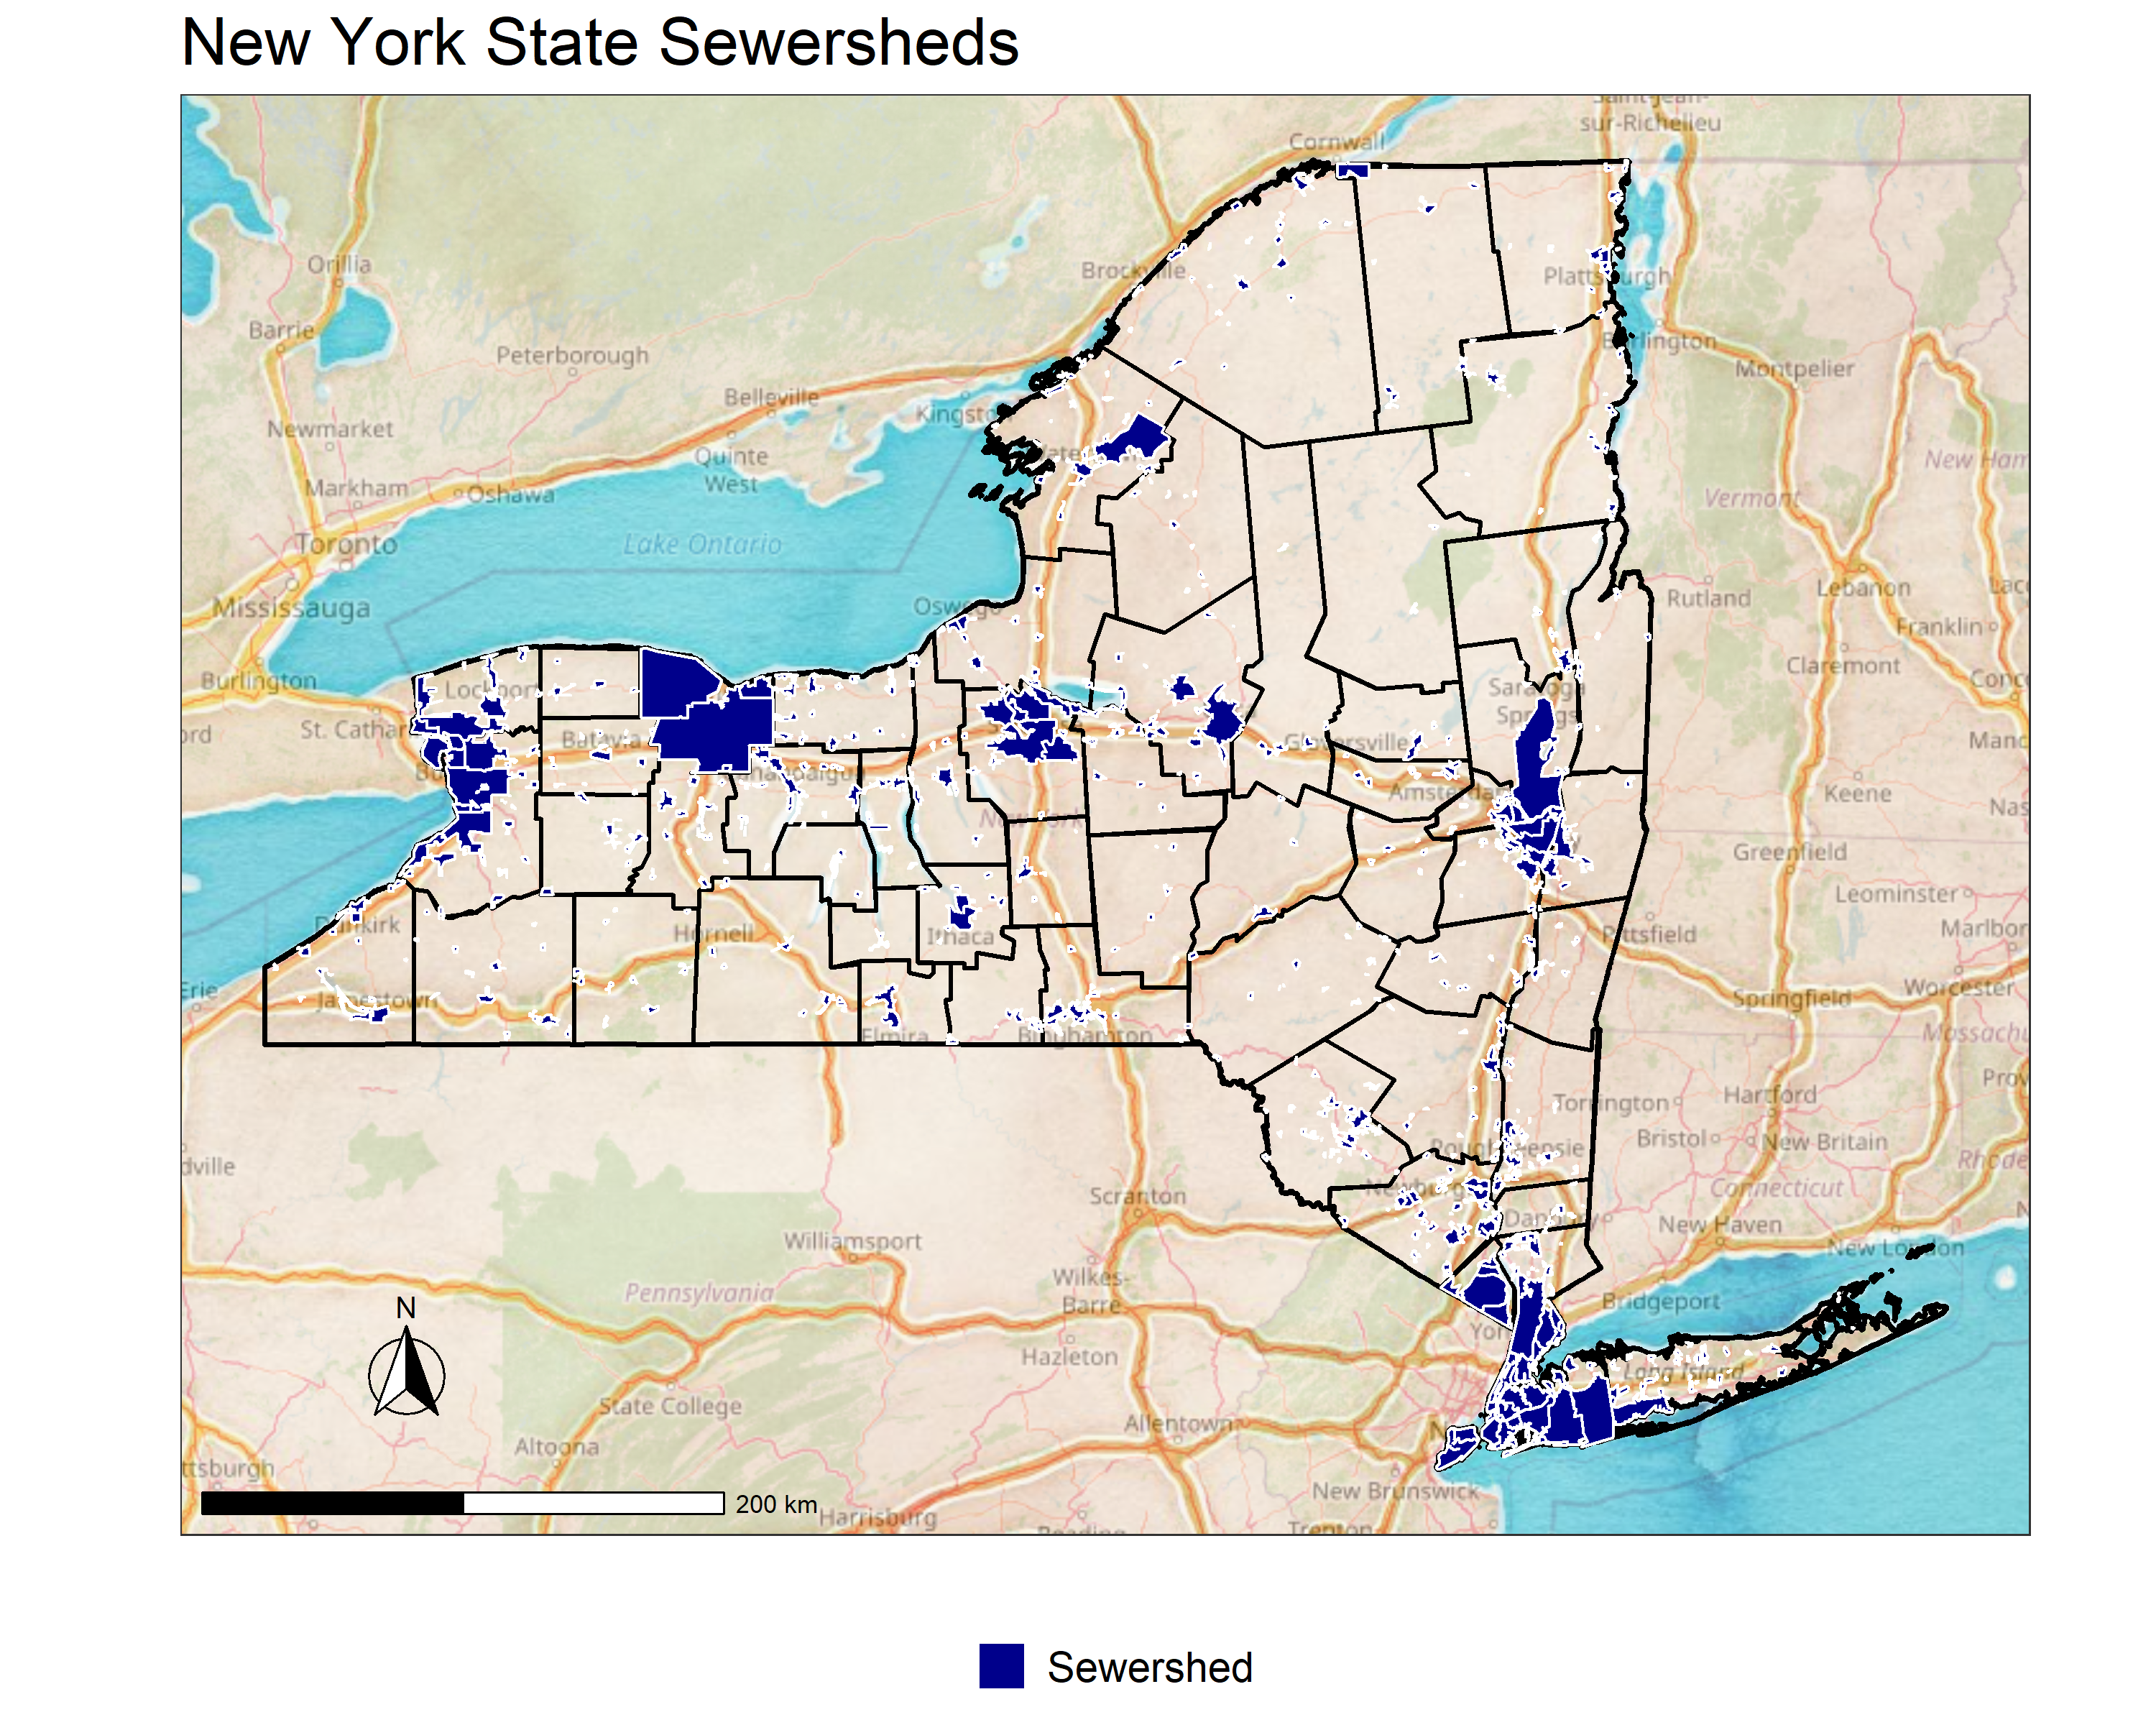
\includegraphics[width=41.67in]{Images/Map-stamen3} 

}

\caption{New York State Municipal Sewersheds}\label{fig:fig2}
\end{figure}

In this section, you will learn about how NYS mapped their sewersheds and the open-source methods that were used. This overview will be referenced in future sections and the methods can be applied to other jurisdictions looking to produce maps of sewershed boundaries to aid wastewater surveillance for epidemiology.

\hypertarget{goals-for-this-section}{%
\section{Goals for this section}\label{goals-for-this-section}}

\begin{enumerate}
\def\labelenumi{\arabic{enumi}.}
\item
  Learn about the process that NYS used to map sewersheds.
\item
  Identify methods used to address challenges in mapping and producing ``best'' estimates for sewershed boundaries.
\item
  Learn how NYS is using sewershed boundaries to enhance the utility of wastewater epidemiology.
\end{enumerate}

\hypertarget{resources}{%
\section{Resources}\label{resources}}

\begin{itemize}
\item
  Video powerpoint for how NY created sewersheds.
\item
  Hill, D, Larsen, DA. 2023. \href{https://doi.org/10.1371/journal.pgph.0001062}{Using geographic information systems to link population estimates to wastewater surveillance data in New York State, USA.} PLOS Global Public Health. The paper explains the process for mapping all of NYS's sewersheds including data collection, processing, and estimating population estimates for each sewershed.
\item
  \href{https://www.arcgis.com/home/item.html?id=e795007660ae4a1fae5f86b40d065b3a}{NYS sewershed data (ArcGIS online download)}. Access and download NYS sewershed data to see how data are recorded.
\item
  \href{https://github.com/nys-wwsn/ny-sewer-spatial-data}{NYS sewershed data} (GitHub data download). Access and download NYS sewershed data directly into your R session.
\item
  \href{https://dthill196.github.io/NY-Sewershed-Populations/}{NYS sewershed data viewer}. Visually inspect NYS sewersheds and the population served by each. The page includes example code for downloading and adding population data to sewershed shapefiles in the program R.
\item
  \href{https://desktop.arcgis.com/en/arcmap/latest/manage-data/editing-fundamentals/adding-the-editor-toolbar.htm}{Using the Editor toolbar in ArcGIS}. ArcGIS can be an excellent way to digitally edit spatial data.
\item
  \href{https://r-spatial.org/}{R spatial tools}. R is an open-source program, and most mapping projects and analyses can be completed using the software.
\end{itemize}

\hypertarget{maps-and-spatial-data-for-communities-connected-to-public-sewer}{%
\chapter{Maps and spatial data for communities connected to public sewer}\label{maps-and-spatial-data-for-communities-connected-to-public-sewer}}

\hypertarget{overview}{%
\section{Overview}\label{overview}}

In this section, we will review existing maps for community sewer and how to go about making them. While there is a plethora of digital spatial data on many topics, there is not yet a comprehensive national database for sewers in the United States (US). Prior to the NYS DOH sewershed mapping project, there was also not a comprehensive map of NY's sewer systems. There are, however, some public databases for locations of publicly owned treatment works including permitted wastewater treatment plants. The US Environmental Protection Agency (EPA) maintains records on permitted WWTPs and so do most state environmental offices. Using these public records, we know where the municipal WWTPs are and this provides a starting point for mapping a state's sewer systems. The next step involves collecting data from other sources like:

\begin{itemize}
\tightlist
\item
  State tax parcel records
\item
  Municipal records for local sewer taxes
\item
  WWTP infrastructure maps or engineering design
\item
  County or local planning documents
\item
  Location of manholes or sewer mains
\item
  Lists of addresses for properties that report paying a sewer tax
\end{itemize}

Many of these records will be housed in local GIS, tax, planning, or municipal offices. Some will be public, and others might require permission to access or data use agreements. The final product of mapping a state's sewer systems does not result in any identifiable data being produced, and if you explain to local officials the goals of the project and what the final product will look like, data sharing should not be an issue. Work with your local partners to ensure that their questions are answered, and any concerns are addressed.

\hypertarget{goals-for-this-section-1}{%
\section{Goals for this section}\label{goals-for-this-section-1}}

In this section, you will:

\begin{enumerate}
\def\labelenumi{\arabic{enumi}.}
\tightlist
\item
  Review an example sewershed parcel mapping exercise for one county in New York State
\item
  Explore loading and manipulating maps in ArcGIS and R
\item
  Gather data on your state's WWTP locations
\item
  Contact local offices, WWTP operators, and others to gather data on sewer locations
\item
  Gather parcel property data for your jurisdiction
\end{enumerate}

\hypertarget{resources-1}{%
\section{Resources}\label{resources-1}}

\begin{itemize}
\tightlist
\item
  \href{https://www.arcgis.com/apps/mapviewer/index.html?url=https://services5.arcgis.com/fmKivMCp6fwbWbeE/ArcGIS/rest/services/2023_NSGIC_Parcel_Portal/FeatureServer\&source=sd}{National parcel data viewer} / \href{https://services5.arcgis.com/fmKivMCp6fwbWbeE/ArcGIS/rest/services/2023_NSGIC_Parcel_Portal/FeatureServer}{data access portal}. This is a data portal that lets you explore each state in the US and whether they have tax parcel data. Some links bring you to county or state websites and from there you can view and download the data.
\end{itemize}

ArcGIS tutorials

\begin{itemize}
\item
  \href{https://pro.arcgis.com/en/pro-app/latest/help/data/geodatabases/overview/load-data.htm}{Loading data into Arc}
\item
  \href{https://pro.arcgis.com/en/pro-app/latest/get-started/create-points-from-a-table.htm}{Add point data from a table}
\item
  \href{https://desktop.arcgis.com/en/arcmap/latest/manage-data/editing-fundamentals/adding-the-editor-toolbar.htm}{Using the Editor tool}
\item
  \href{https://pro.arcgis.com/en/pro-app/latest/help/data/geodatabases/overview/export-data.htm}{Save your shapefile}
\end{itemize}

Q GIS tutorials

\begin{itemize}
\item
  \href{https://qgis.org/download/}{Downloading Q}
\item
  \href{https://www.youtube.com/watch?v=WbnFbgE7P4o}{Add polygon data to Q}
\item
  \href{https://qgis-tuts-wu.readthedocs.io/en/latest/land_degradation_development/interpolation/loading_table.html}{Add point data from a table}
\item
  \href{https://docs.qgis.org/3.40/en/docs/user_manual/working_with_vector/editing_geometry_attributes.html}{Edit data in Q}
\item
  \href{https://www.youtube.com/watch?v=Syas8ajiQ8w}{Split multipart polygons}
\item
  \href{https://www.youtube.com/watch?v=bf1w1AeaHsw}{Save your data in Q}
\end{itemize}

\hypertarget{training-exercise}{%
\section{Training exercise}\label{training-exercise}}

This training will show how to use publicly available tax parcel data to draw municipal sewershed boundaries. You will need to download R to run this script on your machine.

For this example, we are going to map sewersheds in Onondaga County, NY. Sewersheds are the area of land that a wastewater treatment plant (WWTP) serves and include public and private properties. Many states, including NY, keep track of residential and commercial sewer access in their state tax records. We will use data downloaded from the NYS Tax Parcel system for Onondaga county.

You can access the file for Onondaga County at the following location: \href{https://data.gis.ny.gov/datasets/sharegisny::nys-tax-parcels-public/about?layer=1}{NYS Tax Parcel Data}. These data are very large, so for the purposes of this tutorial, I have already downloaded the data and filtered for Onondaga County.

You will also need a list of the municipal wastewater treatment plants for Onondaga County. NYS keeps a record of all permitted WWTPs in the state. You can download the file \href{https://data.ny.gov/Energy-Environment/Wastewater-Treatment-Plants/2v6p-juki/about_data}{here}.

We will be able to use these data to:

\begin{enumerate}
\def\labelenumi{\arabic{enumi})}
\item
  Map WWTPs in Onondaga County, NY
\item
  Select parcels that are on public sewer
\item
  Link groups of parcels to the town or village they are within
\item
  Estimate sewershed locations for nearby WWTPs
\end{enumerate}

A note before proceeding: Parcel data are very large and your R session might slow down during some processing steps.

\hypertarget{data-you-will-need-for-this-tutorial}{%
\subsubsection{Data you will need for this tutorial}\label{data-you-will-need-for-this-tutorial}}

You will need to download the following data files for this tutorial (they are stored with this tutorial).

\begin{itemize}
\item
  Onondaga County tax parcels
\item
  NYS WWTP list
\item
  NY county boundaries
\item
  NY town boundaries
\item
  NY village boundaries
\end{itemize}

\hypertarget{step-1---install-and-load-the-necessary-r-packages}{%
\subsection{Step 1 - Install and load the necessary R packages}\label{step-1---install-and-load-the-necessary-r-packages}}

Install packages to your computer.

\begin{Shaded}
\begin{Highlighting}[]
\FunctionTok{install.packages}\NormalTok{(}\StringTok{"gridExtra"}\NormalTok{)}
\FunctionTok{install.packages}\NormalTok{(}\StringTok{"nngeo"}\NormalTok{)}
\FunctionTok{install.packages}\NormalTok{(}\StringTok{"sf"}\NormalTok{)}
\FunctionTok{install.packages}\NormalTok{(}\StringTok{"dplyr"}\NormalTok{)}
\FunctionTok{install.packages}\NormalTok{(}\StringTok{"ggplot2"}\NormalTok{)}
\FunctionTok{install.packages}\NormalTok{(}\StringTok{"tigris"}\NormalTok{)}
\end{Highlighting}
\end{Shaded}

Load packages into your current R session.

\begin{Shaded}
\begin{Highlighting}[]
\FunctionTok{library}\NormalTok{(gridExtra)}
\FunctionTok{library}\NormalTok{(nngeo)}
\FunctionTok{library}\NormalTok{(sf)}
\FunctionTok{library}\NormalTok{(dplyr)}
\FunctionTok{library}\NormalTok{(ggplot2)}
\FunctionTok{library}\NormalTok{(tigris)}
\end{Highlighting}
\end{Shaded}

\hypertarget{step-2---load-the-data-into-your-r-session}{%
\subsection{Step 2 - Load the data into your R session}\label{step-2---load-the-data-into-your-r-session}}

\begin{Shaded}
\begin{Highlighting}[]
\CommentTok{\# Onondaga county tax parcels}
\NormalTok{onondaga\_parcels }\OtherTok{\textless{}{-}} 
  \FunctionTok{st\_read}\NormalTok{(}\StringTok{"E:/Data/ny\_parcels/onondaga\_2020\_Tax\_Parcels\_SHP\_2106/onondaga\_2020\_Tax\_Parcels\_SHP\_2106.shp"}\NormalTok{)}

\CommentTok{\# NY WWTPS}
\NormalTok{ny\_wwtps }\OtherTok{\textless{}{-}} \FunctionTok{read.csv}\NormalTok{(}\StringTok{"data/Wastewater\_Treatment\_Plants\_20250121.csv"}\NormalTok{)}

\CommentTok{\# NY county boundaries {-} for assistance with mapping}
\NormalTok{ny\_counties }\OtherTok{\textless{}{-}} 
  \FunctionTok{st\_read}\NormalTok{(}\StringTok{"E:/Dropbox/CEMI/Wastewater/Data/NYS\_Civil\_Boundaries.shp/Counties\_Shoreline.shp"}\NormalTok{)}

\CommentTok{\# Filter for Onondaga county}
\NormalTok{onondaga\_border }\OtherTok{\textless{}{-}}\NormalTok{ ny\_counties }\SpecialCharTok{\%\textgreater{}\%}
  \FunctionTok{filter}\NormalTok{(NAME }\SpecialCharTok{==} \StringTok{"Onondaga"}\NormalTok{)}

\CommentTok{\# nys town, city, village boundaries}
\NormalTok{towns }\OtherTok{\textless{}{-}} 
  \FunctionTok{st\_read}\NormalTok{(}\StringTok{"E:/Dropbox/CEMI/Wastewater/Data/NYS\_Civil\_Boundaries.shp/Cities\_Towns.shp"}\NormalTok{)}

\CommentTok{\# Onondaga towns}
\NormalTok{onondaga\_towns }\OtherTok{\textless{}{-}}\NormalTok{ towns }\SpecialCharTok{\%\textgreater{}\%}
  \FunctionTok{filter}\NormalTok{(COUNTY }\SpecialCharTok{==} \StringTok{"Onondaga"}\NormalTok{)}

\CommentTok{\# villages}
\NormalTok{villages }\OtherTok{\textless{}{-}} 
  \FunctionTok{st\_read}\NormalTok{(}\StringTok{"E:/Dropbox/CEMI/Wastewater/Data/NYS\_Civil\_Boundaries.shp/Villages.shp"}\NormalTok{)}

\CommentTok{\# Onondaga villages}
\NormalTok{onondaga\_villages }\OtherTok{\textless{}{-}}\NormalTok{ villages }\SpecialCharTok{\%\textgreater{}\%}
  \FunctionTok{filter}\NormalTok{(COUNTY }\SpecialCharTok{==} \StringTok{"Onondaga"}\NormalTok{)}
\end{Highlighting}
\end{Shaded}

\hypertarget{step-3---filter-the-wwtp-data-for-municipal-sites-only}{%
\subsection{Step 3 - Filter the WWTP data for municipal sites only}\label{step-3---filter-the-wwtp-data-for-municipal-sites-only}}

\begin{Shaded}
\begin{Highlighting}[]
\CommentTok{\# municipal sites only}
\NormalTok{wwtp\_mun }\OtherTok{\textless{}{-}}\NormalTok{ ny\_wwtps }\SpecialCharTok{\%\textgreater{}\%}
  \FunctionTok{filter}\NormalTok{(Plant.Type }\SpecialCharTok{==} \StringTok{"Municipal"}\NormalTok{)}

\CommentTok{\# make the data spatial for mapping purposes using the coordinates in the file}
\NormalTok{wwtp\_mun\_sf }\OtherTok{\textless{}{-}} 
  \FunctionTok{st\_as\_sf}\NormalTok{(wwtp\_mun,}
           \AttributeTok{coords =}  \FunctionTok{c}\NormalTok{(}\StringTok{"Longitude"}\NormalTok{, }\StringTok{"Latitude"}\NormalTok{),}
           \AttributeTok{crs =} \StringTok{"+proj=longlat +datum=WGS84 +no\_defs +ellps=WGS84"}\NormalTok{)}

\CommentTok{\# transform to the same CRS as the Onondaga parcels}
\NormalTok{wwtp\_mun\_sf }\OtherTok{\textless{}{-}} \FunctionTok{st\_transform}\NormalTok{(wwtp\_mun\_sf, }\FunctionTok{st\_crs}\NormalTok{(onondaga\_border))}

\CommentTok{\# filter for Onondaga plants only using st\_intersection}
\NormalTok{wwtp\_onondaga\_sf }\OtherTok{\textless{}{-}} \FunctionTok{st\_intersection}\NormalTok{(wwtp\_mun\_sf, onondaga\_border)}

\CommentTok{\# Map out the plants}
\FunctionTok{ggplot}\NormalTok{()}\SpecialCharTok{+}
  \FunctionTok{geom\_sf}\NormalTok{(}\AttributeTok{data =}\NormalTok{ onondaga\_border, }\AttributeTok{fill =} \ConstantTok{NA}\NormalTok{)}\SpecialCharTok{+}
  \FunctionTok{geom\_sf}\NormalTok{(}\AttributeTok{data =}\NormalTok{ onondaga\_towns, }\AttributeTok{fill =} \StringTok{"dodgerblue"}\NormalTok{, }\AttributeTok{color =} \StringTok{"white"}\NormalTok{)}\SpecialCharTok{+}
  \FunctionTok{geom\_sf}\NormalTok{(}\AttributeTok{data =}\NormalTok{ onondaga\_villages, }\AttributeTok{fill =} \StringTok{"orange"}\NormalTok{, }\AttributeTok{color =} \StringTok{"white"}\NormalTok{)}\SpecialCharTok{+}
  \FunctionTok{geom\_sf}\NormalTok{(}\AttributeTok{data =}\NormalTok{ wwtp\_onondaga\_sf, }\AttributeTok{color =} \StringTok{"black"}\NormalTok{, }\AttributeTok{size =} \DecValTok{3}\NormalTok{)}\SpecialCharTok{+}
  \FunctionTok{theme\_void}\NormalTok{()}
\end{Highlighting}
\end{Shaded}

\includegraphics{_main_files/figure-latex/wwtp data prep-1.pdf}

We can see that many WWTPs fall within village or town boundaries. This should help us differentiate the plants that serve different communities. We can also ask the municipalities and local WWTP operators to learn more, but for now, let us assume that we are not sure.

\hypertarget{step-4---filter-the-parcel-data-for-public-sewer-only}{%
\subsection{Step 4 - Filter the parcel data for public sewer only}\label{step-4---filter-the-parcel-data-for-public-sewer-only}}

There are two fields in the data for sewer. One is the \texttt{SEWER\_TYPE} and the other is \texttt{SEWER\_DESC}. \texttt{SEWER\_DESC} includes three categories: Comm/public, None, or Private. We will filter for the Comm/public sewer parcels only.

\begin{Shaded}
\begin{Highlighting}[]
\CommentTok{\# filter for public sewer parcels}
\FunctionTok{table}\NormalTok{(onondaga\_parcels}\SpecialCharTok{$}\NormalTok{SEWER\_DESC)}
\end{Highlighting}
\end{Shaded}

\begin{verbatim}
## 
## Comm/public        None     Private 
##      138461       11440       30452
\end{verbatim}

\begin{Shaded}
\begin{Highlighting}[]
\NormalTok{onondaga\_sewer }\OtherTok{\textless{}{-}}\NormalTok{ onondaga\_parcels }\SpecialCharTok{\%\textgreater{}\%}
  \FunctionTok{filter}\NormalTok{(SEWER\_DESC }\SpecialCharTok{==} \StringTok{"Comm/public"}\NormalTok{)}

\CommentTok{\# plot the parcel data}
\CommentTok{\# }\AlertTok{NOTE}\CommentTok{ {-} this will take a moment, there are over 100,000 records}
\FunctionTok{ggplot}\NormalTok{()}\SpecialCharTok{+}
  \FunctionTok{geom\_sf}\NormalTok{(}\AttributeTok{data =}\NormalTok{ onondaga\_border, }\AttributeTok{fill =} \ConstantTok{NA}\NormalTok{)}\SpecialCharTok{+}
  \FunctionTok{geom\_sf}\NormalTok{(}\AttributeTok{data =}\NormalTok{ onondaga\_towns, }\AttributeTok{fill =} \StringTok{"dodgerblue"}\NormalTok{, }\AttributeTok{color =} \StringTok{"white"}\NormalTok{)}\SpecialCharTok{+}
  \FunctionTok{geom\_sf}\NormalTok{(}\AttributeTok{data =}\NormalTok{ onondaga\_villages, }\AttributeTok{fill =} \StringTok{"orange"}\NormalTok{, }\AttributeTok{color =} \StringTok{"white"}\NormalTok{)}\SpecialCharTok{+}
  \FunctionTok{geom\_sf}\NormalTok{(}\AttributeTok{data =}\NormalTok{ onondaga\_sewer, }\AttributeTok{color =} \ConstantTok{NA}\NormalTok{, }\AttributeTok{alpha =} \FloatTok{0.5}\NormalTok{)}\SpecialCharTok{+}
  \FunctionTok{geom\_sf}\NormalTok{(}\AttributeTok{data =}\NormalTok{ wwtp\_onondaga\_sf, }\AttributeTok{color =} \StringTok{"black"}\NormalTok{, }\AttributeTok{size =} \DecValTok{3}\NormalTok{)}\SpecialCharTok{+}
  \FunctionTok{theme\_void}\NormalTok{()}\SpecialCharTok{+}
  \FunctionTok{labs}\NormalTok{(}\AttributeTok{title =} \StringTok{"Onondaga county parcels connected to public sewer"}\NormalTok{)}
\end{Highlighting}
\end{Shaded}

\includegraphics{_main_files/figure-latex/parcel data prep-1.pdf}

\hypertarget{step-5---link-sewer-parcels-to-towns-and-villages}{%
\subsection{Step 5 - Link sewer parcels to towns and villages}\label{step-5---link-sewer-parcels-to-towns-and-villages}}

\begin{Shaded}
\begin{Highlighting}[]
\CommentTok{\# cut out the village boundaries from the towns}
\NormalTok{town\_no\_village }\OtherTok{\textless{}{-}}\FunctionTok{st\_difference}\NormalTok{(onondaga\_towns, }\FunctionTok{st\_combine}\NormalTok{(onondaga\_villages))}

\CommentTok{\# intersect the villages/towns with the sewer parcels}
\NormalTok{sewer\_town\_intersection }\OtherTok{\textless{}{-}} \FunctionTok{st\_intersection}\NormalTok{(onondaga\_sewer, town\_no\_village)}
\NormalTok{sewer\_village\_intersection }\OtherTok{\textless{}{-}} \FunctionTok{st\_intersection}\NormalTok{(onondaga\_sewer, onondaga\_villages)}

\CommentTok{\# group by town / village unit and dissolve}
\CommentTok{\# Note we are using a buffer to help remove extra spaces and lines between }
\CommentTok{\# parcels}

\CommentTok{\# first we buffer}
\NormalTok{dissolved\_towns }\OtherTok{\textless{}{-}}\NormalTok{ sewer\_town\_intersection }\SpecialCharTok{\%\textgreater{}\%}
  \FunctionTok{st\_as\_sf}\NormalTok{() }\SpecialCharTok{\%\textgreater{}\%}
  \FunctionTok{st\_buffer}\NormalTok{(}\DecValTok{100}\NormalTok{)}

\CommentTok{\# then dissolve}
\NormalTok{dissolved\_towns }\OtherTok{\textless{}{-}}\NormalTok{ dissolved\_towns }\SpecialCharTok{\%\textgreater{}\%} 
  \FunctionTok{group\_by}\NormalTok{(NAME) }\SpecialCharTok{\%\textgreater{}\%} \CommentTok{\# name of the town}
  \FunctionTok{summarise}\NormalTok{() }\SpecialCharTok{\%\textgreater{}\%}
  \FunctionTok{ungroup}\NormalTok{()}

\CommentTok{\# remove the buffer distance}
\NormalTok{dissolved\_towns }\OtherTok{\textless{}{-}}\NormalTok{ dissolved\_towns }\SpecialCharTok{\%\textgreater{}\%}
  \FunctionTok{st\_buffer}\NormalTok{(}\SpecialCharTok{{-}}\DecValTok{100}\NormalTok{) }

\CommentTok{\# villages}

\CommentTok{\# first we buffer}
\NormalTok{dissolved\_villages }\OtherTok{\textless{}{-}}\NormalTok{ sewer\_village\_intersection }\SpecialCharTok{\%\textgreater{}\%}
  \FunctionTok{st\_as\_sf}\NormalTok{() }\SpecialCharTok{\%\textgreater{}\%}
  \FunctionTok{st\_buffer}\NormalTok{(}\DecValTok{100}\NormalTok{)}

\CommentTok{\# then dissolve}
\NormalTok{dissolved\_villages }\OtherTok{\textless{}{-}}\NormalTok{ dissolved\_villages }\SpecialCharTok{\%\textgreater{}\%} 
  \FunctionTok{group\_by}\NormalTok{(NAME) }\SpecialCharTok{\%\textgreater{}\%}
  \FunctionTok{summarise}\NormalTok{() }\SpecialCharTok{\%\textgreater{}\%}
  \FunctionTok{ungroup}\NormalTok{()}

\CommentTok{\# remove the buffer distance}
\NormalTok{dissolved\_villages }\OtherTok{\textless{}{-}}\NormalTok{ dissolved\_villages }\SpecialCharTok{\%\textgreater{}\%}
  \FunctionTok{st\_buffer}\NormalTok{(}\SpecialCharTok{{-}}\DecValTok{100}\NormalTok{)}

\CommentTok{\# plot to see how they look}
\FunctionTok{ggplot}\NormalTok{()}\SpecialCharTok{+}
  \FunctionTok{geom\_sf}\NormalTok{(}\AttributeTok{data =}\NormalTok{ onondaga\_border, }\AttributeTok{fill =} \ConstantTok{NA}\NormalTok{)}\SpecialCharTok{+}
  \FunctionTok{geom\_sf}\NormalTok{(}\AttributeTok{data =}\NormalTok{ dissolved\_towns, }\AttributeTok{color =} \StringTok{"white"}\NormalTok{, }\FunctionTok{aes}\NormalTok{(}\AttributeTok{fill =} \StringTok{\textasciigrave{}}\AttributeTok{NAME}\StringTok{\textasciigrave{}}\NormalTok{))}\SpecialCharTok{+}
    \FunctionTok{geom\_sf}\NormalTok{(}\AttributeTok{data =}\NormalTok{ dissolved\_villages, }\AttributeTok{color =} \StringTok{"white"}\NormalTok{, }\FunctionTok{aes}\NormalTok{(}\AttributeTok{fill =} \StringTok{\textasciigrave{}}\AttributeTok{NAME}\StringTok{\textasciigrave{}}\NormalTok{))}\SpecialCharTok{+}
  \FunctionTok{geom\_sf}\NormalTok{(}\AttributeTok{data =}\NormalTok{ wwtp\_onondaga\_sf, }\AttributeTok{size =} \DecValTok{3}\NormalTok{, }\AttributeTok{color =} \StringTok{"black"}\NormalTok{)}\SpecialCharTok{+}
  \FunctionTok{theme\_void}\NormalTok{()}\SpecialCharTok{+}
  \FunctionTok{theme}\NormalTok{(}\AttributeTok{legend.position =} \StringTok{"none"}\NormalTok{)}
\end{Highlighting}
\end{Shaded}

\includegraphics{_main_files/figure-latex/towns -1.pdf}

We now have two layers, parcels in each town or city that are on sewer and parcels in each village that are on sewer. The next step can be to take these data to a local county planning office and identify which town sewer systems go to each plant, then group the polygons to create the sewershed for that plant.

Alternatively, let's do a little more work to make that next step easier. You will notice there are a lot of wayward parcels (parcels that are not near any WWTP or town and look like small ``islands''). They likely flow into nearby systems a little ways off. Also, there are a lot of holes in the parcel groups. We will fill in those holes and then intersect the town and village sewer parcels with census blocks to get more robust geometries for the sewersheds. These steps will make using these data for epidemiology a little easier. If you want to keep the more skeletal boundaries for sewers, you can save that data for future reference.

\hypertarget{clean-up-sewershed-boundaries}{%
\subsubsection{Clean up sewershed boundaries}\label{clean-up-sewershed-boundaries}}

\begin{Shaded}
\begin{Highlighting}[]
\CommentTok{\# remove holes}

\NormalTok{dissolved\_towns\_filled }\OtherTok{\textless{}{-}}\NormalTok{ nngeo}\SpecialCharTok{::}\FunctionTok{st\_remove\_holes}\NormalTok{(dissolved\_towns)}
\NormalTok{dissolved\_villages\_filled }\OtherTok{\textless{}{-}}\NormalTok{ nngeo}\SpecialCharTok{::}\FunctionTok{st\_remove\_holes}\NormalTok{(dissolved\_villages)}

\NormalTok{sewer\_parcel\_plot }\OtherTok{\textless{}{-}} 
  \FunctionTok{ggplot}\NormalTok{()}\SpecialCharTok{+}
  \FunctionTok{geom\_sf}\NormalTok{(}\AttributeTok{data =}\NormalTok{ onondaga\_border, }\AttributeTok{fill =} \ConstantTok{NA}\NormalTok{)}\SpecialCharTok{+}
  \FunctionTok{geom\_sf}\NormalTok{(}\AttributeTok{data =}\NormalTok{ dissolved\_towns\_filled, }\AttributeTok{color =} \StringTok{"white"}\NormalTok{, }\FunctionTok{aes}\NormalTok{(}\AttributeTok{fill =}\NormalTok{ NAME))}\SpecialCharTok{+}
  \FunctionTok{geom\_sf}\NormalTok{(}\AttributeTok{data =}\NormalTok{ dissolved\_villages\_filled, }\AttributeTok{color =} \StringTok{"white"}\NormalTok{, }\FunctionTok{aes}\NormalTok{(}\AttributeTok{fill =}\NormalTok{ NAME))}\SpecialCharTok{+}
  \FunctionTok{geom\_sf}\NormalTok{(}\AttributeTok{data =}\NormalTok{ wwtp\_onondaga\_sf, }\AttributeTok{size =} \DecValTok{3}\NormalTok{, }\AttributeTok{color =} \StringTok{"black"}\NormalTok{)}\SpecialCharTok{+}
  \FunctionTok{labs}\NormalTok{(}\AttributeTok{title =} \StringTok{"Town and village parcels that are on sewer"}\NormalTok{)}\SpecialCharTok{+}
  \FunctionTok{theme\_void}\NormalTok{()}\SpecialCharTok{+}
  \FunctionTok{theme}\NormalTok{(}\AttributeTok{legend.position =} \StringTok{"none"}\NormalTok{,}
        \AttributeTok{plot.title =} \FunctionTok{element\_text}\NormalTok{(}\AttributeTok{hjust =} \FloatTok{0.5}\NormalTok{))}

\NormalTok{sewer\_parcel\_plot}
\end{Highlighting}
\end{Shaded}

\includegraphics{_main_files/figure-latex/remove holes-1.pdf}

\hypertarget{step-6---assign-polygons-to-wwtps}{%
\subsection{Step 6 - Assign polygons to WWTPs}\label{step-6---assign-polygons-to-wwtps}}

We want to now bring our village and town parcel polygons together into one shapefile layer and link the polygons to the nearest WWTP.

\begin{Shaded}
\begin{Highlighting}[]
\CommentTok{\# combine village and town parcels into on R data object}
\NormalTok{village\_town\_sewer }\OtherTok{\textless{}{-}} \FunctionTok{bind\_rows}\NormalTok{(}
\NormalTok{                                dissolved\_towns\_filled, }
\NormalTok{                                dissolved\_villages\_filled}
\NormalTok{                                )}


\CommentTok{\# assign each polygon to a point based on proximity}
\NormalTok{near }\OtherTok{\textless{}{-}} \FunctionTok{st\_nearest\_feature}\NormalTok{(village\_town\_sewer, wwtp\_onondaga\_sf)}

\CommentTok{\# using the row numbers for the nearest feature, we can begin to create some }
\CommentTok{\# sewershed boundaries}
\NormalTok{wwtp\_onondaga\_sf}\SpecialCharTok{$}\NormalTok{wwtp\_row\_id }\OtherTok{\textless{}{-}} \FunctionTok{seq}\NormalTok{(}\DecValTok{1}\SpecialCharTok{:}\FunctionTok{nrow}\NormalTok{(wwtp\_onondaga\_sf))}
\NormalTok{village\_town\_sewer}\SpecialCharTok{$}\NormalTok{parcel\_row\_id }\OtherTok{\textless{}{-}} \FunctionTok{seq}\NormalTok{(}\DecValTok{1}\SpecialCharTok{:}\FunctionTok{nrow}\NormalTok{(village\_town\_sewer))}

\CommentTok{\# combine the list of near wwtps with the Onondaga sewer dataset}
\NormalTok{near\_df }\OtherTok{\textless{}{-}} \FunctionTok{as.data.frame}\NormalTok{(}\FunctionTok{cbind}\NormalTok{(village\_town\_sewer, near))}

\CommentTok{\# rename near value to be the wwtp\_row\_id}
\NormalTok{near\_df}\SpecialCharTok{$}\NormalTok{wwtp\_row\_id }\OtherTok{\textless{}{-}}\NormalTok{ near\_df}\SpecialCharTok{$}\NormalTok{near}

\CommentTok{\# to avoid extra "lines" in our dissolved polygons, we buffer the parcels first}

\CommentTok{\# first we buffer}
\NormalTok{dissolved }\OtherTok{\textless{}{-}}\NormalTok{ near\_df }\SpecialCharTok{\%\textgreater{}\%}
  \FunctionTok{st\_as\_sf}\NormalTok{() }\SpecialCharTok{\%\textgreater{}\%}
  \FunctionTok{st\_buffer}\NormalTok{(}\DecValTok{10}\NormalTok{)}

\CommentTok{\# then dissolve}
\NormalTok{dissolved }\OtherTok{\textless{}{-}}\NormalTok{ dissolved }\SpecialCharTok{\%\textgreater{}\%} 
  \FunctionTok{group\_by}\NormalTok{(wwtp\_row\_id) }\SpecialCharTok{\%\textgreater{}\%}
  \FunctionTok{summarise}\NormalTok{() }\SpecialCharTok{\%\textgreater{}\%}
  \FunctionTok{ungroup}\NormalTok{()}

\CommentTok{\# remove the buffer distance}
\NormalTok{dissolved }\OtherTok{\textless{}{-}}\NormalTok{ dissolved }\SpecialCharTok{\%\textgreater{}\%}
  \FunctionTok{st\_buffer}\NormalTok{(}\SpecialCharTok{{-}}\DecValTok{10}\NormalTok{) }

\CommentTok{\# add the wwtp metadata}
\NormalTok{onondaga\_meta }\OtherTok{\textless{}{-}}\NormalTok{ wwtp\_onondaga\_sf }\SpecialCharTok{\%\textgreater{}\%}
  \FunctionTok{st\_drop\_geometry}\NormalTok{() }

\NormalTok{dissolved }\OtherTok{\textless{}{-}}\NormalTok{ dissolved }\SpecialCharTok{\%\textgreater{}\%}
  \FunctionTok{left\_join}\NormalTok{(onondaga\_meta, }\AttributeTok{by =} \FunctionTok{c}\NormalTok{(}\StringTok{"wwtp\_row\_id"}\NormalTok{))}

\CommentTok{\# plot to see how they look}
\FunctionTok{ggplot}\NormalTok{()}\SpecialCharTok{+}
  \FunctionTok{geom\_sf}\NormalTok{(}\AttributeTok{data =}\NormalTok{ onondaga\_border, }\AttributeTok{fill =} \ConstantTok{NA}\NormalTok{)}\SpecialCharTok{+}
  \FunctionTok{geom\_sf}\NormalTok{(}\AttributeTok{data =}\NormalTok{ dissolved, }\AttributeTok{color =} \StringTok{"darkblue"}\NormalTok{, }\FunctionTok{aes}\NormalTok{(}\AttributeTok{fill =} \StringTok{\textasciigrave{}}\AttributeTok{Facility.Name}\StringTok{\textasciigrave{}}\NormalTok{))}\SpecialCharTok{+}
  \FunctionTok{geom\_sf}\NormalTok{(}\AttributeTok{data =}\NormalTok{ wwtp\_onondaga\_sf, }\AttributeTok{size =} \DecValTok{3}\NormalTok{, }\AttributeTok{color =} \StringTok{"black"}\NormalTok{)}\SpecialCharTok{+}
  \FunctionTok{theme\_void}\NormalTok{()}\SpecialCharTok{+}
  \FunctionTok{theme}\NormalTok{(}\AttributeTok{legend.position =} \StringTok{"bottom"}\NormalTok{)}\SpecialCharTok{+}
  \FunctionTok{guides}\NormalTok{(}\AttributeTok{fill =} \FunctionTok{guide\_legend}\NormalTok{(}\AttributeTok{nrow =} \DecValTok{4}\NormalTok{, }\AttributeTok{byrow=}\ConstantTok{TRUE}\NormalTok{))}\SpecialCharTok{+}
  \FunctionTok{scale\_fill\_manual}\NormalTok{(}\AttributeTok{values =}\NormalTok{ MetBrewer}\SpecialCharTok{::}\FunctionTok{met.brewer}\NormalTok{(}\AttributeTok{name =} \StringTok{"Nizami"}\NormalTok{, }\AttributeTok{n =} \DecValTok{11}\NormalTok{),}
                    \AttributeTok{labels =} \ControlFlowTok{function}\NormalTok{(x) stringr}\SpecialCharTok{::}\FunctionTok{str\_wrap}\NormalTok{(x, }\AttributeTok{width =} \DecValTok{15}\NormalTok{))}
\end{Highlighting}
\end{Shaded}

\includegraphics{_main_files/figure-latex/link parcel polys to points-1.pdf}

We can save these R objects as shapefiles.

\begin{Shaded}
\begin{Highlighting}[]
\FunctionTok{st\_write}\NormalTok{(dissolved\_towns\_filled, }
         \AttributeTok{dsn =} \StringTok{"data/onondaga town sewer parcels/onondaga town sewer parcels.shp"}\NormalTok{)}

\FunctionTok{st\_write}\NormalTok{(dissolved\_villages\_filled, }
         \AttributeTok{dsn =} \StringTok{"data/onondaga village sewer parcels/onondaga village sewer parcels.shp"}\NormalTok{)}

\FunctionTok{st\_write}\NormalTok{(dissolved, }
         \AttributeTok{dsn =} \StringTok{"data/town village sewer parcels/town village sewer parcels.shp"}\NormalTok{)}
\end{Highlighting}
\end{Shaded}

\hypertarget{training-review}{%
\section{Training review}\label{training-review}}

We have used publicly available tax parcel data to estimate sewersheds for municipal WWTPs in Onondaga County, NY. The boundaries are not exact nor are they complete. You will need to work with local planning offices to improve the boundary estimates and finalize assigning each polygon to the WWTP that they flow into.

Some additional data you might gather to create the final boundaries include municipal tax roles, municipal sewer infrastructure maps or GIS data, or your tax parcel data might have what in NY is called a ``Special Districts'' table.

\hypertarget{appendix-1---special-districts}{%
\subsection{Appendix 1 - Special districts}\label{appendix-1---special-districts}}

The Special Districts table is a dataset that includes more detail on each tax parcel like what water and fire district the parcel is part of. These tables are not always publicly available and you might need permission to work with these data. If you can obtain these data, you can merge the special districts to the parcel data using the municipal tax parcel ID, and then group and filter by special district names for sewer districts. Not all special district table will have sewer data, but many will.

\hypertarget{appendix-2---create-polygons-using-census-blocks}{%
\subsection{Appendix 2 - create polygons using census blocks}\label{appendix-2---create-polygons-using-census-blocks}}

We can also draw sewershed boundaries using census blocks. By intersecting census blocks with sewer parcels, we can map the parts of each town and village on sewer.

An advantage to including the entire block that intersects with a sewershed parcel is that it will make merging these data with census population data easier in the future. Obtaining accurate population estimates for the number of people on sewer is an important part of wastewater-based epidemiology.

\hypertarget{download-censusblocks-for-nys}{%
\subsubsection{Download censusblocks for NYS}\label{download-censusblocks-for-nys}}

\begin{Shaded}
\begin{Highlighting}[]
\NormalTok{b }\OtherTok{\textless{}{-}}\NormalTok{ tigris}\SpecialCharTok{::}\FunctionTok{blocks}\NormalTok{(}\AttributeTok{state =} \StringTok{"New York"}\NormalTok{, }\AttributeTok{county =} \StringTok{"Onondaga"}\NormalTok{, }\AttributeTok{year =} \DecValTok{2020}\NormalTok{)}
\end{Highlighting}
\end{Shaded}

\begin{Shaded}
\begin{Highlighting}[]
\CommentTok{\# blocks that intersect with town sewer parcels}
\CommentTok{\# transform crs to match}
\NormalTok{b }\OtherTok{\textless{}{-}} \FunctionTok{st\_transform}\NormalTok{(b, }\FunctionTok{st\_crs}\NormalTok{(dissolved\_towns\_filled))}

\NormalTok{town\_sewer\_b }\OtherTok{\textless{}{-}} \FunctionTok{st\_intersects}\NormalTok{(b, dissolved\_towns\_filled)}
\NormalTok{town\_sewer\_b }\OtherTok{\textless{}{-}} \FunctionTok{as.data.frame}\NormalTok{(town\_sewer\_b)}

\CommentTok{\# blocks that intersect with village sewer parcels}
\NormalTok{village\_sewer\_b }\OtherTok{\textless{}{-}} \FunctionTok{st\_intersects}\NormalTok{(b, dissolved\_villages\_filled)}
\NormalTok{village\_sewer\_b }\OtherTok{\textless{}{-}} \FunctionTok{as.data.frame}\NormalTok{(village\_sewer\_b)}

\CommentTok{\# add row ids and then select for row ids in the intersection}
\NormalTok{b}\SpecialCharTok{$}\NormalTok{b\_row\_id }\OtherTok{\textless{}{-}} \FunctionTok{seq}\NormalTok{(}\DecValTok{1}\SpecialCharTok{:}\FunctionTok{nrow}\NormalTok{(b))}

\NormalTok{village\_sewer\_blocks }\OtherTok{\textless{}{-}}\NormalTok{ b }\SpecialCharTok{\%\textgreater{}\%} 
  \FunctionTok{filter}\NormalTok{(b\_row\_id }\SpecialCharTok{\%in\%}\NormalTok{ village\_sewer\_b}\SpecialCharTok{$}\NormalTok{row.id)}
\NormalTok{town\_sewer\_blocks }\OtherTok{\textless{}{-}}\NormalTok{ b }\SpecialCharTok{\%\textgreater{}\%}
   \FunctionTok{filter}\NormalTok{(b\_row\_id }\SpecialCharTok{\%in\%}\NormalTok{ town\_sewer\_b}\SpecialCharTok{$}\NormalTok{row.id)}

\CommentTok{\# add town / village sewer }
\NormalTok{dissolved\_towns\_filled}\SpecialCharTok{$}\NormalTok{town\_id }\OtherTok{\textless{}{-}} \FunctionTok{seq}\NormalTok{(}\DecValTok{1}\SpecialCharTok{:}\FunctionTok{nrow}\NormalTok{(dissolved\_towns\_filled))}
\NormalTok{dissolved\_villages\_filled}\SpecialCharTok{$}\NormalTok{village\_id }\OtherTok{\textless{}{-}} \FunctionTok{seq}\NormalTok{(}\DecValTok{1}\SpecialCharTok{:}\FunctionTok{nrow}\NormalTok{(dissolved\_villages\_filled))}

\NormalTok{village\_sewer\_b }\OtherTok{\textless{}{-}}\NormalTok{ village\_sewer\_b }\SpecialCharTok{\%\textgreater{}\%}
  \FunctionTok{rename}\NormalTok{(}\AttributeTok{village\_id =}\NormalTok{ col.id,}
         \AttributeTok{b\_row\_id =}\NormalTok{ row.id) }\SpecialCharTok{\%\textgreater{}\%}
  \FunctionTok{left\_join}\NormalTok{(dissolved\_villages\_filled, }\AttributeTok{by =} \FunctionTok{c}\NormalTok{(}\StringTok{"village\_id"}\NormalTok{)) }\SpecialCharTok{\%\textgreater{}\%}
  \FunctionTok{st\_drop\_geometry}\NormalTok{() }\SpecialCharTok{\%\textgreater{}\%}
  \FunctionTok{select}\NormalTok{(}\SpecialCharTok{{-}}\NormalTok{geometry)}

\CommentTok{\# add to village\_sewer\_blocks}
\NormalTok{village\_sewer\_blocks }\OtherTok{\textless{}{-}} \FunctionTok{left\_join}\NormalTok{(village\_sewer\_blocks, village\_sewer\_b, }
                                  \AttributeTok{by =} \FunctionTok{c}\NormalTok{(}\StringTok{"b\_row\_id"}\NormalTok{)}
\NormalTok{                                  )}

\CommentTok{\# group by village and dissolve}

\CommentTok{\# first we buffer}
\NormalTok{village\_sewer\_blocks }\OtherTok{\textless{}{-}}\NormalTok{ village\_sewer\_blocks }\SpecialCharTok{\%\textgreater{}\%}
  \FunctionTok{st\_as\_sf}\NormalTok{() }\SpecialCharTok{\%\textgreater{}\%}
  \FunctionTok{st\_buffer}\NormalTok{(}\DecValTok{100}\NormalTok{)}

\CommentTok{\# then dissolve}
\NormalTok{village\_sewer\_blocks }\OtherTok{\textless{}{-}}\NormalTok{ village\_sewer\_blocks }\SpecialCharTok{\%\textgreater{}\%} 
  \FunctionTok{group\_by}\NormalTok{(NAME) }\SpecialCharTok{\%\textgreater{}\%}
  \FunctionTok{summarise}\NormalTok{() }\SpecialCharTok{\%\textgreater{}\%}
  \FunctionTok{ungroup}\NormalTok{()}

\CommentTok{\# remove the buffer distance}
\NormalTok{village\_sewer\_blocks }\OtherTok{\textless{}{-}}\NormalTok{ village\_sewer\_blocks }\SpecialCharTok{\%\textgreater{}\%}
  \FunctionTok{st\_buffer}\NormalTok{(}\SpecialCharTok{{-}}\DecValTok{100}\NormalTok{)}

\DocumentationTok{\#\# repeat for towns}

\NormalTok{town\_sewer\_b }\OtherTok{\textless{}{-}}\NormalTok{ town\_sewer\_b }\SpecialCharTok{\%\textgreater{}\%}
  \FunctionTok{rename}\NormalTok{(}\AttributeTok{town\_id =}\NormalTok{ col.id,}
         \AttributeTok{b\_row\_id =}\NormalTok{ row.id) }\SpecialCharTok{\%\textgreater{}\%}
  \FunctionTok{left\_join}\NormalTok{(dissolved\_towns\_filled, }\AttributeTok{by =} \FunctionTok{c}\NormalTok{(}\StringTok{"town\_id"}\NormalTok{)) }\SpecialCharTok{\%\textgreater{}\%}
  \FunctionTok{st\_drop\_geometry}\NormalTok{() }\SpecialCharTok{\%\textgreater{}\%}
  \FunctionTok{select}\NormalTok{(}\SpecialCharTok{{-}}\NormalTok{geometry)}

\CommentTok{\# add to village\_sewer\_blocks}
\NormalTok{town\_sewer\_blocks }\OtherTok{\textless{}{-}} \FunctionTok{left\_join}\NormalTok{(town\_sewer\_blocks, town\_sewer\_b, }
                               \AttributeTok{by =} \FunctionTok{c}\NormalTok{(}\StringTok{"b\_row\_id"}\NormalTok{)}
\NormalTok{                               )}

\CommentTok{\# group by village and dissolve}

\CommentTok{\# first we buffer}
\NormalTok{town\_sewer\_blocks }\OtherTok{\textless{}{-}}\NormalTok{ town\_sewer\_blocks }\SpecialCharTok{\%\textgreater{}\%}
  \FunctionTok{st\_as\_sf}\NormalTok{() }\SpecialCharTok{\%\textgreater{}\%}
  \FunctionTok{st\_buffer}\NormalTok{(}\DecValTok{100}\NormalTok{)}

\CommentTok{\# then dissolve}
\NormalTok{town\_sewer\_blocks }\OtherTok{\textless{}{-}}\NormalTok{ town\_sewer\_blocks }\SpecialCharTok{\%\textgreater{}\%} 
  \FunctionTok{group\_by}\NormalTok{(NAME) }\SpecialCharTok{\%\textgreater{}\%}
  \FunctionTok{summarise}\NormalTok{() }\SpecialCharTok{\%\textgreater{}\%}
  \FunctionTok{ungroup}\NormalTok{()}

\CommentTok{\# remove the buffer distance}
\NormalTok{town\_sewer\_blocks }\OtherTok{\textless{}{-}}\NormalTok{ town\_sewer\_blocks }\SpecialCharTok{\%\textgreater{}\%}
  \FunctionTok{st\_buffer}\NormalTok{(}\SpecialCharTok{{-}}\DecValTok{100}\NormalTok{)}

\CommentTok{\# fill holes}
\NormalTok{town\_sewer\_blocks\_filled }\OtherTok{\textless{}{-}}\NormalTok{ nngeo}\SpecialCharTok{::}\FunctionTok{st\_remove\_holes}\NormalTok{(town\_sewer\_blocks)}
\NormalTok{village\_sewer\_blocks\_filled }\OtherTok{\textless{}{-}}\NormalTok{ nngeo}\SpecialCharTok{::}\FunctionTok{st\_remove\_holes}\NormalTok{(village\_sewer\_blocks)}

\NormalTok{block\_sewer\_plot }\OtherTok{\textless{}{-}}
  \FunctionTok{ggplot}\NormalTok{()}\SpecialCharTok{+}
  \FunctionTok{geom\_sf}\NormalTok{(}\AttributeTok{data =}\NormalTok{ onondaga\_border, }\AttributeTok{fill =} \ConstantTok{NA}\NormalTok{)}\SpecialCharTok{+}
  \FunctionTok{geom\_sf}\NormalTok{(}\AttributeTok{data =}\NormalTok{ village\_sewer\_blocks\_filled, }\AttributeTok{color =} \StringTok{"white"}\NormalTok{,}
          \FunctionTok{aes}\NormalTok{(}\AttributeTok{fill =}\NormalTok{ NAME)}
\NormalTok{          )}\SpecialCharTok{+}
  \FunctionTok{geom\_sf}\NormalTok{(}\AttributeTok{data =}\NormalTok{ town\_sewer\_blocks\_filled, }\AttributeTok{color =} \StringTok{"white"}\NormalTok{,}
          \FunctionTok{aes}\NormalTok{(}\AttributeTok{fill =}\NormalTok{ NAME)}
\NormalTok{          )}\SpecialCharTok{+}
  \FunctionTok{geom\_sf}\NormalTok{(}\AttributeTok{data =}\NormalTok{ wwtp\_onondaga\_sf, }\AttributeTok{size =} \DecValTok{3}\NormalTok{, }\AttributeTok{color =} \StringTok{"black"}\NormalTok{)}\SpecialCharTok{+}
  \FunctionTok{labs}\NormalTok{(}\AttributeTok{title =} \StringTok{"Town and  village blocks that intersect with}\SpecialCharTok{\textbackslash{}n}\StringTok{parcels on sewer"}\NormalTok{)}\SpecialCharTok{+}
  \FunctionTok{theme\_void}\NormalTok{()}\SpecialCharTok{+}
  \FunctionTok{theme}\NormalTok{(}\AttributeTok{legend.position =} \StringTok{"none"}\NormalTok{,}
        \AttributeTok{plot.title =} \FunctionTok{element\_text}\NormalTok{(}\AttributeTok{hjust =} \FloatTok{0.5}\NormalTok{))}

\CommentTok{\# block\_sewer\_plot}
\end{Highlighting}
\end{Shaded}

So now we have two sets of data to bring to the local planning offices or WWTP operators to help in creating the final boundaries. Let's take a look at them side by side.

\begin{Shaded}
\begin{Highlighting}[]
\NormalTok{gridExtra}\SpecialCharTok{::}\FunctionTok{grid.arrange}\NormalTok{(sewer\_parcel\_plot, block\_sewer\_plot, }\AttributeTok{nrow =} \DecValTok{1}\NormalTok{)}
\end{Highlighting}
\end{Shaded}

\includegraphics{_main_files/figure-latex/final maps-1.pdf}

We can also link these data to the nearest WWTP like we did for parcels.

\begin{Shaded}
\begin{Highlighting}[]
\CommentTok{\# combine into one object}
\NormalTok{village\_town\_blocks }\OtherTok{\textless{}{-}} \FunctionTok{bind\_rows}\NormalTok{(town\_sewer\_blocks, village\_sewer\_blocks)}

\CommentTok{\# assign each polygon to a point based on proximity}
\NormalTok{near }\OtherTok{\textless{}{-}} \FunctionTok{st\_nearest\_feature}\NormalTok{(village\_town\_blocks, wwtp\_onondaga\_sf)}

\CommentTok{\# using the rownumbers for the nearest feature, we can begin to create some }
\CommentTok{\# sewershed boundaries}
\NormalTok{wwtp\_onondaga\_sf}\SpecialCharTok{$}\NormalTok{wwtp\_row\_id }\OtherTok{\textless{}{-}} \FunctionTok{seq}\NormalTok{(}\DecValTok{1}\SpecialCharTok{:}\FunctionTok{nrow}\NormalTok{(wwtp\_onondaga\_sf))}
\NormalTok{village\_town\_blocks}\SpecialCharTok{$}\NormalTok{parcel\_row\_id }\OtherTok{\textless{}{-}} \FunctionTok{seq}\NormalTok{(}\DecValTok{1}\SpecialCharTok{:}\FunctionTok{nrow}\NormalTok{(village\_town\_blocks))}

\CommentTok{\# combine the list of near wwtps with the onondaga sewer dataset}
\NormalTok{near\_df }\OtherTok{\textless{}{-}} \FunctionTok{as.data.frame}\NormalTok{(}\FunctionTok{cbind}\NormalTok{(village\_town\_blocks, near))}

\CommentTok{\# rename near value to be the wwtp\_row\_id}
\NormalTok{near\_df}\SpecialCharTok{$}\NormalTok{wwtp\_row\_id }\OtherTok{\textless{}{-}}\NormalTok{ near\_df}\SpecialCharTok{$}\NormalTok{near}

\CommentTok{\# to avoid extra "lines" in our dissolved polygons, we buffer the parcels first}

\CommentTok{\# first we buffer}
\NormalTok{dissolved }\OtherTok{\textless{}{-}}\NormalTok{ near\_df }\SpecialCharTok{\%\textgreater{}\%}
  \FunctionTok{st\_as\_sf}\NormalTok{() }\SpecialCharTok{\%\textgreater{}\%}
  \FunctionTok{st\_buffer}\NormalTok{(}\DecValTok{10}\NormalTok{)}

\CommentTok{\# then dissolve}
\NormalTok{dissolved }\OtherTok{\textless{}{-}}\NormalTok{ dissolved }\SpecialCharTok{\%\textgreater{}\%} 
  \FunctionTok{group\_by}\NormalTok{(wwtp\_row\_id) }\SpecialCharTok{\%\textgreater{}\%}
  \FunctionTok{summarise}\NormalTok{() }\SpecialCharTok{\%\textgreater{}\%}
  \FunctionTok{ungroup}\NormalTok{()}

\CommentTok{\# remove the buffer distance}
\NormalTok{dissolved }\OtherTok{\textless{}{-}}\NormalTok{ dissolved }\SpecialCharTok{\%\textgreater{}\%}
  \FunctionTok{st\_buffer}\NormalTok{(}\SpecialCharTok{{-}}\DecValTok{10}\NormalTok{) }

\CommentTok{\# add the wwtp metadata}
\NormalTok{onondaga\_meta }\OtherTok{\textless{}{-}}\NormalTok{ wwtp\_onondaga\_sf }\SpecialCharTok{\%\textgreater{}\%}
  \FunctionTok{st\_drop\_geometry}\NormalTok{() }

\NormalTok{dissolved }\OtherTok{\textless{}{-}}\NormalTok{ dissolved }\SpecialCharTok{\%\textgreater{}\%}
  \FunctionTok{left\_join}\NormalTok{(onondaga\_meta, }\AttributeTok{by =} \FunctionTok{c}\NormalTok{(}\StringTok{"wwtp\_row\_id"}\NormalTok{))}

\CommentTok{\# plot to see how they look}
\FunctionTok{ggplot}\NormalTok{()}\SpecialCharTok{+}
  \FunctionTok{geom\_sf}\NormalTok{(}\AttributeTok{data =}\NormalTok{ onondaga\_border, }\AttributeTok{fill =} \ConstantTok{NA}\NormalTok{)}\SpecialCharTok{+}
  \FunctionTok{geom\_sf}\NormalTok{(}\AttributeTok{data =}\NormalTok{ dissolved, }\AttributeTok{color =} \StringTok{"darkblue"}\NormalTok{, }\FunctionTok{aes}\NormalTok{(}\AttributeTok{fill =} \StringTok{\textasciigrave{}}\AttributeTok{Facility.Name}\StringTok{\textasciigrave{}}\NormalTok{))}\SpecialCharTok{+}
  \FunctionTok{geom\_sf}\NormalTok{(}\AttributeTok{data =}\NormalTok{ wwtp\_onondaga\_sf, }\AttributeTok{size =} \DecValTok{3}\NormalTok{, }\AttributeTok{color =} \StringTok{"black"}\NormalTok{)}\SpecialCharTok{+}
  \FunctionTok{theme\_void}\NormalTok{()}\SpecialCharTok{+}
  \FunctionTok{theme}\NormalTok{(}\AttributeTok{legend.position =} \StringTok{"none"}\NormalTok{)}
\end{Highlighting}
\end{Shaded}

\includegraphics{_main_files/figure-latex/village blocks-1.pdf}

\hypertarget{appendix-3---polygons-from-point-data}{%
\subsection{Appendix 3 - Polygons from point data}\label{appendix-3---polygons-from-point-data}}

Some datasets may be made up of points like manhole locations or points for each parcel connected to a sewer system. You can create a polygon from point data using the following code.

\begin{Shaded}
\begin{Highlighting}[]
\CommentTok{\# change parcels to centroids}
\NormalTok{onondaga\_sewer\_centroids }\OtherTok{\textless{}{-}} \FunctionTok{st\_centroid}\NormalTok{(onondaga\_sewer)}

\CommentTok{\# find the nearest wwtp for each sewer parcel}
\NormalTok{near }\OtherTok{\textless{}{-}} \FunctionTok{st\_nearest\_feature}\NormalTok{(onondaga\_sewer\_centroids, wwtp\_onondaga\_sf)}

\CommentTok{\# using the row numbers for the nearest feature, we can begin to create some }
\CommentTok{\# sewershed boundaries}
\NormalTok{wwtp\_onondaga\_sf}\SpecialCharTok{$}\NormalTok{wwtp\_row\_id }\OtherTok{\textless{}{-}} \FunctionTok{seq}\NormalTok{(}\DecValTok{1}\SpecialCharTok{:}\FunctionTok{nrow}\NormalTok{(wwtp\_onondaga\_sf))}
\NormalTok{onondaga\_sewer\_centroids}\SpecialCharTok{$}\NormalTok{parcel\_row\_id }\OtherTok{\textless{}{-}} \FunctionTok{seq}\NormalTok{(}\DecValTok{1}\SpecialCharTok{:}\FunctionTok{nrow}\NormalTok{(onondaga\_sewer\_centroids))}

\CommentTok{\# combine the list of near wwtps with the Onondaga sewer dataset}
\NormalTok{near\_df }\OtherTok{\textless{}{-}} \FunctionTok{as.data.frame}\NormalTok{(}\FunctionTok{cbind}\NormalTok{(onondaga\_sewer\_centroids, near))}

\CommentTok{\# rename near value to be the wwtp\_row\_id}
\NormalTok{near\_df}\SpecialCharTok{$}\NormalTok{wwtp\_row\_id }\OtherTok{\textless{}{-}}\NormalTok{ near\_df}\SpecialCharTok{$}\NormalTok{near}

\CommentTok{\# plot the points}
\FunctionTok{ggplot}\NormalTok{()}\SpecialCharTok{+}
  \FunctionTok{geom\_sf}\NormalTok{(}\AttributeTok{data =}\NormalTok{ onondaga\_border, }\AttributeTok{fill =} \ConstantTok{NA}\NormalTok{)}\SpecialCharTok{+}
  \FunctionTok{geom\_sf}\NormalTok{(}\AttributeTok{data =} \FunctionTok{st\_as\_sf}\NormalTok{(near\_df), }\AttributeTok{alpha =} \FloatTok{0.5}\NormalTok{)}\SpecialCharTok{+}
  \FunctionTok{theme\_void}\NormalTok{()}
\end{Highlighting}
\end{Shaded}

\includegraphics{_main_files/figure-latex/polygons from point data-1.pdf}

\begin{Shaded}
\begin{Highlighting}[]
\CommentTok{\# make a buffer around each point}
\NormalTok{near\_df }\OtherTok{\textless{}{-}}\NormalTok{ near\_df }\SpecialCharTok{\%\textgreater{}\%}
  \FunctionTok{st\_as\_sf}\NormalTok{() }\SpecialCharTok{\%\textgreater{}\%}
  \FunctionTok{st\_buffer}\NormalTok{(}\AttributeTok{dist =} \DecValTok{100}\NormalTok{) }\CommentTok{\# you might need to play with this buffer distance}

\CommentTok{\# group by wwtp\_row\_id and merge into polygons}
\CommentTok{\# then dissolve}
\NormalTok{dissolved }\OtherTok{\textless{}{-}}\NormalTok{ near\_df }\SpecialCharTok{\%\textgreater{}\%} 
  \FunctionTok{group\_by}\NormalTok{(wwtp\_row\_id) }\SpecialCharTok{\%\textgreater{}\%}
  \FunctionTok{summarise}\NormalTok{() }\SpecialCharTok{\%\textgreater{}\%}
  \FunctionTok{ungroup}\NormalTok{()}

\CommentTok{\# plot}
\FunctionTok{ggplot}\NormalTok{()}\SpecialCharTok{+}
  \FunctionTok{geom\_sf}\NormalTok{(}\AttributeTok{data =}\NormalTok{ onondaga\_border, }\AttributeTok{fill =} \ConstantTok{NA}\NormalTok{)}\SpecialCharTok{+}
  \FunctionTok{geom\_sf}\NormalTok{(}\AttributeTok{data =}\NormalTok{ dissolved, }\FunctionTok{aes}\NormalTok{(}\AttributeTok{fill =} \FunctionTok{as.factor}\NormalTok{(wwtp\_row\_id)))}\SpecialCharTok{+}
  \FunctionTok{geom\_sf}\NormalTok{(}\AttributeTok{data =}\NormalTok{ wwtp\_onondaga\_sf, }\FunctionTok{aes}\NormalTok{(}\AttributeTok{size =} \StringTok{\textasciigrave{}}\AttributeTok{Average.Design.Hydraulic.Flow}\StringTok{\textasciigrave{}}\NormalTok{))}\SpecialCharTok{+}
  \FunctionTok{theme\_void}\NormalTok{()}\SpecialCharTok{+}
  \FunctionTok{theme}\NormalTok{(}\AttributeTok{legend.position =} \StringTok{"none"}\NormalTok{)}
\end{Highlighting}
\end{Shaded}

\includegraphics{_main_files/figure-latex/polygons from points continued-1.pdf}

You can then fill the holes like we did before or do some additional cleaning in ArcGIS or from the special districts tables.

\hypertarget{adding-census-data-to-wastewater-based-epidemiology}{%
\chapter{Adding Census Data to Wastewater-Based Epidemiology}\label{adding-census-data-to-wastewater-based-epidemiology}}

\hypertarget{overview-1}{%
\section{Overview}\label{overview-1}}

Wastewater-based epidemiology (WBE) data can be enhanced by adding other public data sources. One source is United States Census (US Census) data, which can add population demographic variables to WBE data, This vignette demonstrates how to take a spatial WBE dataset of sewershed boundaries in New York State (NYS) and add US Census data using spatial intersection methods.

\hypertarget{install-and-load-r-packages}{%
\subsection{Install and Load R packages}\label{install-and-load-r-packages}}

Install packages to your computer.

\begin{Shaded}
\begin{Highlighting}[]
\FunctionTok{install.packages}\NormalTok{(}\StringTok{"dplyr"}\NormalTok{)}
\FunctionTok{install.packages}\NormalTok{(}\StringTok{"ggplot2"}\NormalTok{)}
\FunctionTok{install.packages}\NormalTok{(}\StringTok{"sf"}\NormalTok{)}
\FunctionTok{install.packages}\NormalTok{(}\StringTok{"tidycensus"}\NormalTok{)}
\FunctionTok{install.packages}\NormalTok{(}\StringTok{"units"}\NormalTok{)}
\end{Highlighting}
\end{Shaded}

Load packages into your R session.

\begin{Shaded}
\begin{Highlighting}[]
\FunctionTok{library}\NormalTok{(dplyr) }\CommentTok{\# data wrangling}
\FunctionTok{library}\NormalTok{(sf) }\CommentTok{\# spatial data manipulation}
\FunctionTok{library}\NormalTok{(ggplot2) }\CommentTok{\# making plots and maps}
\FunctionTok{library}\NormalTok{(tidycensus) }\CommentTok{\# download tabular census data}
\FunctionTok{library}\NormalTok{(tigris) }\CommentTok{\# download spatial census data}
\FunctionTok{library}\NormalTok{(tidyr) }\CommentTok{\# data wrangling}
\FunctionTok{library}\NormalTok{(units) }\CommentTok{\# handling variables with unit assignment}
\end{Highlighting}
\end{Shaded}

\hypertarget{load-wastewater-data}{%
\section{Load wastewater data}\label{load-wastewater-data}}

Sewershed boundaries for NYS can be downloaded from \href{https://www.arcgis.com/home/item.html?id=e795007660ae4a1fae5f86b40d065b3a}{ArcGIS online}.

\begin{Shaded}
\begin{Highlighting}[]
\CommentTok{\# load the boundaries}
\NormalTok{sewersheds }\OtherTok{\textless{}{-}} \FunctionTok{st\_read}\NormalTok{(}\StringTok{"data/New York State Sewersheds/New York State Sewersheds.shp"}\NormalTok{)}

\CommentTok{\# select the variables we want to keep}
\NormalTok{sewersheds }\OtherTok{\textless{}{-}}\NormalTok{ sewersheds }\SpecialCharTok{\%\textgreater{}\%}
\NormalTok{  dplyr}\SpecialCharTok{::}\FunctionTok{select}\NormalTok{(County, City, WWTP\_ID, WWTP, Sewershed, SW\_ID, geometry)}
\end{Highlighting}
\end{Shaded}

Map your data.

\begin{Shaded}
\begin{Highlighting}[]
\CommentTok{\# plot to view the data}
\FunctionTok{ggplot}\NormalTok{()}\SpecialCharTok{+}
  \FunctionTok{geom\_sf}\NormalTok{(}\AttributeTok{data =}\NormalTok{ sewersheds, }\AttributeTok{fill =} \StringTok{"white"}\NormalTok{, }\AttributeTok{color =} \StringTok{"black"}\NormalTok{)}\SpecialCharTok{+}
  \FunctionTok{theme\_void}\NormalTok{()}
\end{Highlighting}
\end{Shaded}

\includegraphics{_main_files/figure-latex/plot sewersheds-1.pdf}

\hypertarget{load-us-census-data-method---tidy-census}{%
\section{Load US Census data method - Tidy Census}\label{load-us-census-data-method---tidy-census}}

US Census data can be added to your R session using the packages \texttt{tidycensus} and \texttt{tigris}. Both packages connect to the US Census API for downloading tabular data or spatial boundaries. You will need an API key to access the data. For information on obtaining a key, visit the \texttt{tidycensus} \href{https://walker-data.com/tidycensus/reference/census_api_key.html}{website}.

\begin{Shaded}
\begin{Highlighting}[]
\CommentTok{\# retrieve your API key if stored in the environment}
\FunctionTok{census\_api\_key}\NormalTok{(}\FunctionTok{Sys.getenv}\NormalTok{(}\StringTok{\textquotesingle{}CENSUS\_API\_KEY\textquotesingle{}}\NormalTok{))}
\end{Highlighting}
\end{Shaded}

For this example, we are going to download 2020 decennial census data and calculate the total number of individuals that self-identify as black or African American from that year. We will calculate totals and percentage of total population. We are going to use census tracts as our geography.

To download the data, we need to know the name of the variables we want and for that, we use the \texttt{load\_variables} command.

\begin{Shaded}
\begin{Highlighting}[]
\CommentTok{\# load the variable names into an R object. cache = TRUE can speed the data download step in the next portion}
\NormalTok{census\_var\_names }\OtherTok{\textless{}{-}} \FunctionTok{load\_variables}\NormalTok{(}\AttributeTok{year =} \DecValTok{2020}\NormalTok{, }\AttributeTok{dataset =} \StringTok{"pl"}\NormalTok{, }\AttributeTok{cache =} \ConstantTok{TRUE}\NormalTok{)}
\end{Highlighting}
\end{Shaded}

\begin{Shaded}
\begin{Highlighting}[]
\CommentTok{\# look at the first few rows of data}
\FunctionTok{head}\NormalTok{(census\_var\_names)}
\end{Highlighting}
\end{Shaded}

\begin{verbatim}
## # A tibble: 6 x 3
##   name    label                                             concept         
##   <chr>   <chr>                                             <chr>           
## 1 H1_001N " !!Total:"                                       OCCUPANCY STATUS
## 2 H1_002N " !!Total:!!Occupied"                             OCCUPANCY STATUS
## 3 H1_003N " !!Total:!!Vacant"                               OCCUPANCY STATUS
## 4 P1_001N " !!Total:"                                       RACE            
## 5 P1_002N " !!Total:!!Population of one race:"              RACE            
## 6 P1_003N " !!Total:!!Population of one race:!!White alone" RACE
\end{verbatim}

This function can load the variable names for many datasets from the US Census and provides the name, the variable description, and the concept group that the variable is part of. Looking at the options, we can see that we want a variable from the \texttt{RACE} concept, specifically, \texttt{P1\_004N}, which is ``!!Total:!!Population of one race:!!Black or African American alone''. For this exercise, we will not be included those that identify as multiple racial or ethnic groups, but you can adapt the methods presented to make those calculations.

To get the total for each census tract that identify as black or African American, we need this variable. However, to calculate the percent of the population, we also need the total population, which is the variable '' !!Total:'' or \texttt{P1\_001N}. We will use the \texttt{get\_dencennial} function to download the data into our R session.

\begin{Shaded}
\begin{Highlighting}[]
\CommentTok{\# download the decennial data for the tract geography for NYS}
\NormalTok{census\_data }\OtherTok{\textless{}{-}} \FunctionTok{get\_decennial}\NormalTok{(}
  \AttributeTok{year =} \DecValTok{2020}\NormalTok{,}
  \AttributeTok{geography =} \StringTok{"tract"}\NormalTok{,}
  \AttributeTok{state =} \StringTok{"New York"}\NormalTok{,}
  \AttributeTok{variables =} \FunctionTok{c}\NormalTok{(}
    \FunctionTok{c}\NormalTok{(}\AttributeTok{population\_total =} \StringTok{"P1\_001N"}\NormalTok{),}
    \AttributeTok{black\_alone =} \StringTok{"P1\_004N"}
\NormalTok{  )}
\NormalTok{)}
\end{Highlighting}
\end{Shaded}

\begin{Shaded}
\begin{Highlighting}[]
\CommentTok{\# view the first few rows of data}
\FunctionTok{head}\NormalTok{(census\_data)}
\end{Highlighting}
\end{Shaded}

\begin{verbatim}
## # A tibble: 6 x 4
##   GEOID       NAME                                       variable         value
##   <chr>       <chr>                                      <chr>            <dbl>
## 1 36001000100 Census Tract 1, Albany County, New York    population_total  2073
## 2 36001000201 Census Tract 2.01, Albany County, New York population_total  3125
## 3 36001000202 Census Tract 2.02, Albany County, New York population_total  2598
## 4 36001000301 Census Tract 3.01, Albany County, New York population_total  3190
## 5 36001000302 Census Tract 3.02, Albany County, New York population_total  3496
## 6 36001000401 Census Tract 4.01, Albany County, New York population_total  2216
\end{verbatim}

The resulting dataset is now in our R session with 10,822 rows. We will need to pivot the dataframe to a wider format because it placed the variables in a long format.

\begin{Shaded}
\begin{Highlighting}[]
\CommentTok{\# pivot the data from long to wide format}
\NormalTok{census\_data }\OtherTok{\textless{}{-}} \FunctionTok{pivot\_wider}\NormalTok{(census\_data,}
                           \AttributeTok{names\_from =}\NormalTok{ variable)}

\CommentTok{\# summary of the dataset variables}
\FunctionTok{summary}\NormalTok{(census\_data)}
\end{Highlighting}
\end{Shaded}

\begin{verbatim}
##     GEOID               NAME           population_total  black_alone    
##  Length:5411        Length:5411        Min.   :    0    Min.   :   0.0  
##  Class :character   Class :character   1st Qu.: 2490    1st Qu.:  47.5  
##  Mode  :character   Mode  :character   Median : 3578    Median : 164.0  
##                                        Mean   : 3733    Mean   : 551.9  
##                                        3rd Qu.: 4762    3rd Qu.: 667.0  
##                                        Max.   :17222    Max.   :7935.0
\end{verbatim}

Now we have census counts for individuals that self-identify as black or African American and we want to add these data to our wastewater sewershed boundaries. To do this, we need to add the census geometry (the spatial component) to the R session.

\begin{Shaded}
\begin{Highlighting}[]
\CommentTok{\# download tracts for NY for 2020 and drop the name column}
\NormalTok{tracts }\OtherTok{\textless{}{-}} \FunctionTok{tracts}\NormalTok{(}\AttributeTok{state =} \StringTok{"New York"}\NormalTok{, }\AttributeTok{year =} \DecValTok{2020}\NormalTok{) }\SpecialCharTok{\%\textgreater{}\%} \FunctionTok{select}\NormalTok{(}\SpecialCharTok{{-}}\NormalTok{NAME) }

\CommentTok{\# join the tract geometries to the census data}
\NormalTok{census\_data\_sf }\OtherTok{\textless{}{-}} \FunctionTok{left\_join}\NormalTok{(tracts, census\_data, }\AttributeTok{by =} \FunctionTok{c}\NormalTok{(}\StringTok{"GEOID"}\NormalTok{))}
\end{Highlighting}
\end{Shaded}

\begin{Shaded}
\begin{Highlighting}[]
\CommentTok{\# check the data structure}
\FunctionTok{str}\NormalTok{(census\_data\_sf)}
\end{Highlighting}
\end{Shaded}

\begin{verbatim}
## Classes 'sf' and 'data.frame':   5411 obs. of  15 variables:
##  $ STATEFP         : chr  "36" "36" "36" "36" ...
##  $ COUNTYFP        : chr  "047" "047" "047" "047" ...
##  $ TRACTCE         : chr  "000700" "000900" "001100" "001300" ...
##  $ GEOID           : chr  "36047000700" "36047000900" "36047001100" "36047001300" ...
##  $ NAMELSAD        : chr  "Census Tract 7" "Census Tract 9" "Census Tract 11" "Census Tract 13" ...
##  $ MTFCC           : chr  "G5020" "G5020" "G5020" "G5020" ...
##  $ FUNCSTAT        : chr  "S" "S" "S" "S" ...
##  $ ALAND           : num  176774 163469 168507 293167 154138 ...
##  $ AWATER          : num  0 0 0 0 0 ...
##  $ INTPTLAT        : chr  "+40.6923505" "+40.6917206" "+40.6932903" "+40.6976150" ...
##  $ INTPTLON        : chr  "-073.9973434" "-073.9916018" "-073.9877087" "-073.9883586" ...
##  $ NAME            : chr  "Census Tract 7, Kings County, New York" "Census Tract 9, Kings County, New York" "Census Tract 11, Kings County, New York" "Census Tract 13, Kings County, New York" ...
##  $ population_total: num  4415 5167 1578 2465 1694 ...
##  $ black_alone     : num  151 197 178 234 172 ...
##  $ geometry        :sfc_MULTIPOLYGON of length 5411; first list element: List of 1
##   ..$ :List of 1
##   .. ..$ : num [1:35, 1:2] -74 -74 -74 -74 -74 ...
##   ..- attr(*, "class")= chr [1:3] "XY" "MULTIPOLYGON" "sfg"
##  - attr(*, "sf_column")= chr "geometry"
##  - attr(*, "agr")= Factor w/ 3 levels "constant","aggregate",..: NA NA NA NA NA NA NA NA NA NA ...
##   ..- attr(*, "names")= chr [1:14] "STATEFP" "COUNTYFP" "TRACTCE" "GEOID" ...
\end{verbatim}

\hypertarget{adding-the-census-data-to-the-wastewater-data}{%
\section{Adding the Census data to the wastewater data}\label{adding-the-census-data-to-the-wastewater-data}}

\hypertarget{spatial-transformations}{%
\subsection{Spatial transformations}\label{spatial-transformations}}

To add our population data to the sewershed data, we have a few steps to complete. First, both of our datasets need to be the same spatial projection so that they spatially overlap and can be mapped on top of each other.

\begin{Shaded}
\begin{Highlighting}[]
\CommentTok{\# transform the census data CRS to match the sewersheds}
\NormalTok{census\_data\_sf }\OtherTok{\textless{}{-}} \FunctionTok{st\_transform}\NormalTok{(census\_data\_sf, }\FunctionTok{st\_crs}\NormalTok{(sewersheds))}

\CommentTok{\# plot the data, the layers should overlap}
\FunctionTok{ggplot}\NormalTok{()}\SpecialCharTok{+}
  \FunctionTok{geom\_sf}\NormalTok{(}\AttributeTok{data =}\NormalTok{ census\_data\_sf, }\AttributeTok{fill =} \StringTok{"white"}\NormalTok{, }\AttributeTok{color =} \StringTok{"black"}\NormalTok{)}\SpecialCharTok{+}
  \FunctionTok{geom\_sf}\NormalTok{(}\AttributeTok{data =}\NormalTok{ sewersheds, }\AttributeTok{fill =} \StringTok{"blue"}\NormalTok{, }\AttributeTok{color =} \StringTok{"black"}\NormalTok{)}\SpecialCharTok{+}
  \FunctionTok{theme\_void}\NormalTok{()}
\end{Highlighting}
\end{Shaded}

\includegraphics{_main_files/figure-latex/spatial transformation-1.pdf}

\hypertarget{spatial-intersection}{%
\subsection{Spatial intersection}\label{spatial-intersection}}

Now we want to spatially intersect the data. This will assign census count data to the sewersheds that overlap. Sewershed boundaries do not follow census tract boundaries closely, so we have two options for assigning the data. First, we can apportion census data to the sewersheds using the proportion of each census tract area that is within the sewershed area. Alternatively, we can assign the total population for all intersecting tracts to the sewershed.

The first method, called areal apportionment, is generally thought to provide more accurate methods for counts of the data, but assumes that people are evenly distributed within the census tract. The second method could be useful if it is not known how evenly the population is distributed and you want to avoid excluding anyone. We will practice both methods.

\hypertarget{areal-apportionment}{%
\subsubsection{Areal apportionment}\label{areal-apportionment}}

\begin{Shaded}
\begin{Highlighting}[]
\CommentTok{\# calculate the area of each census tract. Note this field becomes a unit }
\CommentTok{\# variable, we will have to drop those later}
\NormalTok{census\_data\_sf}\SpecialCharTok{$}\NormalTok{tract\_area }\OtherTok{\textless{}{-}} \FunctionTok{st\_area}\NormalTok{(census\_data\_sf)}

\CommentTok{\# turn of spherical geometry to handle overlapping edges and invalid vertices }
\CommentTok{\# warnings}
\NormalTok{sf}\SpecialCharTok{::}\FunctionTok{sf\_use\_s2}\NormalTok{(}\ConstantTok{FALSE}\NormalTok{)}

\CommentTok{\# intersect both datasets, creating a new dataset that has slivers of each tract}
\CommentTok{\# that intersects a sewershed}
\NormalTok{intersection }\OtherTok{\textless{}{-}} \FunctionTok{st\_intersection}\NormalTok{(sewersheds, census\_data\_sf)}

\FunctionTok{summary}\NormalTok{(intersection)}
\end{Highlighting}
\end{Shaded}

\begin{verbatim}
##     County              City             WWTP_ID              WWTP          
##  Length:7963        Length:7963        Length:7963        Length:7963       
##  Class :character   Class :character   Class :character   Class :character  
##  Mode  :character   Mode  :character   Mode  :character   Mode  :character  
##                                                                             
##                                                                             
##                                                                             
##   Sewershed            SW_ID             STATEFP            COUNTYFP        
##  Length:7963        Length:7963        Length:7963        Length:7963       
##  Class :character   Class :character   Class :character   Class :character  
##  Mode  :character   Mode  :character   Mode  :character   Mode  :character  
##                                                                             
##                                                                             
##                                                                             
##    TRACTCE             GEOID             NAMELSAD            MTFCC          
##  Length:7963        Length:7963        Length:7963        Length:7963       
##  Class :character   Class :character   Class :character   Class :character  
##  Mode  :character   Mode  :character   Mode  :character   Mode  :character  
##                                                                             
##                                                                             
##                                                                             
##    FUNCSTAT             ALAND               AWATER            INTPTLAT        
##  Length:7963        Min.   :0.000e+00   Min.   :0.000e+00   Length:7963       
##  Class :character   1st Qu.:2.136e+05   1st Qu.:0.000e+00   Class :character  
##  Mode  :character   Median :1.176e+06   Median :0.000e+00   Mode  :character  
##                     Mean   :1.933e+07   Mean   :2.107e+06                     
##                     3rd Qu.:6.154e+06   3rd Qu.:1.536e+05                     
##                     Max.   :1.828e+09   Max.   :1.997e+09                     
##    INTPTLON             NAME           population_total  black_alone    
##  Length:7963        Length:7963        Min.   :    0    Min.   :   0.0  
##  Class :character   Class :character   1st Qu.: 2593    1st Qu.:  61.0  
##  Mode  :character   Mode  :character   Median : 3672    Median : 211.0  
##                                        Mean   : 3803    Mean   : 587.3  
##                                        3rd Qu.: 4824    3rd Qu.: 734.5  
##                                        Max.   :17222    Max.   :7935.0  
##    tract_area                      geometry   
##  Min.   :2.169e+04   GEOMETRYCOLLECTION:  28  
##  1st Qu.:2.261e+05   MULTIPOLYGON      :1583  
##  Median :1.277e+06   POLYGON           :6352  
##  Mean   :2.140e+07   epsg:4269         :   0  
##  3rd Qu.:6.565e+06   +proj=long...     :   0  
##  Max.   :1.993e+09
\end{verbatim}

Our spatial data are now combined into one spatial data object.

\begin{Shaded}
\begin{Highlighting}[]
\CommentTok{\# calculate a new area for each sliver}
\NormalTok{intersection}\SpecialCharTok{$}\NormalTok{sliver\_area }\OtherTok{\textless{}{-}} \FunctionTok{st\_area}\NormalTok{(intersection)}

\CommentTok{\# calculate the proportion of area that each sliver occupies in the sewershed}
\NormalTok{intersection}\SpecialCharTok{$}\NormalTok{prop\_area }\OtherTok{\textless{}{-}}\NormalTok{ intersection}\SpecialCharTok{$}\NormalTok{sliver\_area }\SpecialCharTok{/}\NormalTok{ intersection}\SpecialCharTok{$}\NormalTok{tract\_area}
\FunctionTok{summary}\NormalTok{(intersection}\SpecialCharTok{$}\NormalTok{prop\_area)}
\end{Highlighting}
\end{Shaded}

\begin{verbatim}
##    Min. 1st Qu.  Median    Mean 3rd Qu.    Max. 
## 0.00000 0.06113 0.88439 0.60984 1.00122 1.00216
\end{verbatim}

\begin{Shaded}
\begin{Highlighting}[]
\CommentTok{\# You will notice some areas are slightly over 1 representing a rounding error. Let\textquotesingle{}s make those all 1 to avoid assignment issues}

\CommentTok{\# drop units}
\NormalTok{intersection}\SpecialCharTok{$}\NormalTok{prop\_area }\OtherTok{\textless{}{-}} \FunctionTok{drop\_units}\NormalTok{(intersection}\SpecialCharTok{$}\NormalTok{prop\_area)}
\NormalTok{intersection}\SpecialCharTok{$}\NormalTok{prop\_area }\OtherTok{\textless{}{-}} \FunctionTok{ifelse}\NormalTok{(intersection}\SpecialCharTok{$}\NormalTok{prop\_area }\SpecialCharTok{\textgreater{}} \DecValTok{1}\NormalTok{, }
                                 \DecValTok{1}\NormalTok{, }
\NormalTok{                                 intersection}\SpecialCharTok{$}\NormalTok{prop\_area}
\NormalTok{                                 )}
\FunctionTok{summary}\NormalTok{(intersection}\SpecialCharTok{$}\NormalTok{prop\_area)}
\end{Highlighting}
\end{Shaded}

\begin{verbatim}
##    Min. 1st Qu.  Median    Mean 3rd Qu.    Max. 
## 0.00000 0.06113 0.88439 0.60930 1.00000 1.00000
\end{verbatim}

\begin{Shaded}
\begin{Highlighting}[]
\CommentTok{\# multiply the proportional area by the totals for black or African American and total population to get proportional values}
\NormalTok{intersection}\SpecialCharTok{$}\NormalTok{prop\_black }\OtherTok{\textless{}{-}}\NormalTok{ intersection}\SpecialCharTok{$}\NormalTok{prop\_area }\SpecialCharTok{*}\NormalTok{ intersection}\SpecialCharTok{$}\NormalTok{black\_alone}
\NormalTok{intersection}\SpecialCharTok{$}\NormalTok{prop\_population }\OtherTok{\textless{}{-}} 
\NormalTok{  intersection}\SpecialCharTok{$}\NormalTok{prop\_area }\SpecialCharTok{*}\NormalTok{ intersection}\SpecialCharTok{$}\NormalTok{population\_total}

\CommentTok{\# how we will group the data by sewershed and sum the total population and total black population in each sewershed}
\NormalTok{intersection\_final }\OtherTok{\textless{}{-}}\NormalTok{ intersection }\SpecialCharTok{\%\textgreater{}\%}
  \FunctionTok{group\_by}\NormalTok{(County, City, WWTP\_ID, WWTP, Sewershed, SW\_ID) }\SpecialCharTok{\%\textgreater{}\%}
  \FunctionTok{summarize}\NormalTok{(}\AttributeTok{sum\_black\_alone =} \FunctionTok{sum}\NormalTok{(prop\_black, }\AttributeTok{na.rm =} \ConstantTok{TRUE}\NormalTok{),}
            \AttributeTok{sum\_total\_population =} \FunctionTok{sum}\NormalTok{(prop\_population)}
\NormalTok{            ) }\SpecialCharTok{\%\textgreater{}\%}
  \FunctionTok{ungroup}\NormalTok{()}

\CommentTok{\# our resulting dataset has 674 rows, one for each sewershed, and proportional estimates for population totals and the total number of individuals that self identify as black or African American}
\FunctionTok{summary}\NormalTok{(intersection\_final)}
\end{Highlighting}
\end{Shaded}

\begin{verbatim}
##     County              City             WWTP_ID              WWTP          
##  Length:674         Length:674         Length:674         Length:674        
##  Class :character   Class :character   Class :character   Class :character  
##  Mode  :character   Mode  :character   Mode  :character   Mode  :character  
##                                                                             
##                                                                             
##                                                                             
##   Sewershed            SW_ID           sum_black_alone     sum_total_population
##  Length:674         Length:674         Min.   :     0.00   Min.   :      0.2   
##  Class :character   Class :character   1st Qu.:     0.74   1st Qu.:     66.6   
##  Mode  :character   Mode  :character   Median :    12.91   Median :    595.6   
##                                        Mean   :  4932.45   Mean   :  27214.5   
##                                        3rd Qu.:   381.10   3rd Qu.:   7356.8   
##                                        Max.   :307461.96   Max.   :1154606.8   
##                geometry  
##  GEOMETRYCOLLECTION:  2  
##  MULTIPOLYGON      :160  
##  POLYGON           :512  
##  epsg:4269         :  0  
##  +proj=long...     :  0  
## 
\end{verbatim}

We have estimated totals, which can be useful, but often, percentage of the population is more informative for analyses. We can get an estimated proportion of the population by dividing the total black alone variable by the total population value.Also, you will notice that the values are no longer integers, meaning that there are estimates for total number of people that include decimals. These can be rounded to the nearest whole number to return the data back to integers.

\begin{Shaded}
\begin{Highlighting}[]
\CommentTok{\# calculate the proportion}
\NormalTok{intersection\_final}\SpecialCharTok{$}\NormalTok{prop\_black }\OtherTok{\textless{}{-}} 
\NormalTok{  intersection\_final}\SpecialCharTok{$}\NormalTok{sum\_black\_alone }\SpecialCharTok{/}\NormalTok{ intersection\_final}\SpecialCharTok{$}\NormalTok{sum\_total\_population}

\CommentTok{\# plot the percentages}
\FunctionTok{ggplot}\NormalTok{()}\SpecialCharTok{+}
  \FunctionTok{geom\_sf}\NormalTok{(}\AttributeTok{data =}\NormalTok{ intersection\_final, }\FunctionTok{aes}\NormalTok{(}\AttributeTok{fill =}\NormalTok{ prop\_black), }\AttributeTok{color =} \StringTok{"black"}\NormalTok{)}\SpecialCharTok{+}
  \FunctionTok{theme\_void}\NormalTok{()}
\end{Highlighting}
\end{Shaded}

\includegraphics{_main_files/figure-latex/areal apportionment 4-1.pdf}

\hypertarget{intersection-assignment}{%
\subsubsection{Intersection assignment}\label{intersection-assignment}}

The other method for assigning data is to assign the total population for all census tracts that intersect with a sewershed.

\begin{Shaded}
\begin{Highlighting}[]
\CommentTok{\# st\_intersects returns a list of the polygon rows that intersect from each }
\CommentTok{\# object}
\NormalTok{intersect\_list }\OtherTok{\textless{}{-}} \FunctionTok{st\_intersects}\NormalTok{(sewersheds, census\_data\_sf)}
\end{Highlighting}
\end{Shaded}

\begin{Shaded}
\begin{Highlighting}[]
\CommentTok{\# make it a dataframe}
\NormalTok{intersect\_df }\OtherTok{\textless{}{-}} \FunctionTok{as.data.frame}\NormalTok{(intersect\_list)}

\CommentTok{\# view the top view rows}
\FunctionTok{head}\NormalTok{(intersect\_df)}
\end{Highlighting}
\end{Shaded}

\begin{verbatim}
##   row.id col.id
## 1      1   1142
## 2      1   1145
## 3      1   1146
## 4      1   2664
## 5      1   3692
## 6      1   5333
\end{verbatim}

Column 1 are the row ids for the sewersheds and column 2 are the row ids for the tracts that intersect them. We will add the row ids to each data object, then use those to merge the census counts to the spatial data and sum to totals.

\begin{Shaded}
\begin{Highlighting}[]
\CommentTok{\# add row ids}
\NormalTok{sewersheds}\SpecialCharTok{$}\NormalTok{sewer\_row\_id }\OtherTok{\textless{}{-}} \FunctionTok{as.integer}\NormalTok{(}\FunctionTok{rownames}\NormalTok{(sewersheds))}
\NormalTok{census\_data\_sf}\SpecialCharTok{$}\NormalTok{census\_row\_id }\OtherTok{\textless{}{-}} \FunctionTok{as.integer}\NormalTok{(}\FunctionTok{rownames}\NormalTok{(census\_data\_sf))}


\CommentTok{\# rename intersect column and merge to spatial sewersheds}
\FunctionTok{colnames}\NormalTok{(intersect\_df) }\OtherTok{\textless{}{-}} \FunctionTok{c}\NormalTok{(}\StringTok{"sewer\_row\_id"}\NormalTok{, }\StringTok{"census\_row\_id"}\NormalTok{)}
\NormalTok{intersect\_combined }\OtherTok{\textless{}{-}} \FunctionTok{full\_join}\NormalTok{(sewersheds, intersect\_df, }
                                \AttributeTok{by =} \FunctionTok{c}\NormalTok{(}\StringTok{"sewer\_row\_id"}\NormalTok{)}
\NormalTok{                                )}

\CommentTok{\# change the census data from a spatial object to a dataframe}
\NormalTok{census\_data\_df }\OtherTok{\textless{}{-}} \FunctionTok{st\_drop\_geometry}\NormalTok{(census\_data\_sf)}

\CommentTok{\# merge census data {-}\textgreater{} note that we have to remove the spatial data from the }
\CommentTok{\# census data}
\NormalTok{intersect\_combined }\OtherTok{\textless{}{-}} \FunctionTok{left\_join}\NormalTok{(intersect\_combined, census\_data\_df, }
                                \AttributeTok{by =} \FunctionTok{c}\NormalTok{(}\StringTok{"census\_row\_id"}\NormalTok{)}
\NormalTok{                                )}

\CommentTok{\# sum the total number of people that are in census tracts intersecting each }
\CommentTok{\# sewershed}
\NormalTok{intersect\_final }\OtherTok{\textless{}{-}}\NormalTok{ intersect\_combined}\SpecialCharTok{\%\textgreater{}\%}
  \FunctionTok{group\_by}\NormalTok{(County, City, WWTP\_ID, WWTP, Sewershed, SW\_ID) }\SpecialCharTok{\%\textgreater{}\%}
  \FunctionTok{summarize}\NormalTok{(}\AttributeTok{sum\_black\_alone =} \FunctionTok{sum}\NormalTok{(black\_alone, }\AttributeTok{na.rm =} \ConstantTok{TRUE}\NormalTok{),}
            \AttributeTok{sum\_total\_population =} \FunctionTok{sum}\NormalTok{(population\_total, }\AttributeTok{na.rm =} \ConstantTok{TRUE}\NormalTok{)}
\NormalTok{            ) }\SpecialCharTok{\%\textgreater{}\%}
  \FunctionTok{ungroup}\NormalTok{()}

\CommentTok{\# calculate the proportions}
\NormalTok{intersect\_final}\SpecialCharTok{$}\NormalTok{prop\_black }\OtherTok{\textless{}{-}} 
\NormalTok{  intersect\_final}\SpecialCharTok{$}\NormalTok{sum\_black\_alone }\SpecialCharTok{/}\NormalTok{ intersect\_final}\SpecialCharTok{$}\NormalTok{sum\_total\_population}

\CommentTok{\# make a map}
\FunctionTok{ggplot}\NormalTok{()}\SpecialCharTok{+}
  \FunctionTok{geom\_sf}\NormalTok{(}\AttributeTok{data =}\NormalTok{ intersect\_final, }\FunctionTok{aes}\NormalTok{(}\AttributeTok{fill =}\NormalTok{ prop\_black), }\AttributeTok{color =} \StringTok{"black"}\NormalTok{)}\SpecialCharTok{+}
  \FunctionTok{theme\_void}\NormalTok{()}
\end{Highlighting}
\end{Shaded}

\includegraphics{_main_files/figure-latex/intersects 3-1.pdf}

\hypertarget{training-review-1}{%
\section{Training review}\label{training-review-1}}

This tutorial demonstrated a process for adding US Census data to WBE spatial data (sewersheds). We calculated the percentage of each sewershed population that identified as black or African American in the 2020 decennial census. These methods can be used to estimate other data available from the US Census. For more information visit the \href{https://www.census.gov/}{US Census website} or \href{https://walker-data.com/tidycensus/}{tidycensus}.

\hypertarget{adding-other-spatial-data-to-wbe}{%
\chapter{Adding other spatial data to WBE}\label{adding-other-spatial-data-to-wbe}}

\hypertarget{overview-2}{%
\section{Overview}\label{overview-2}}

In this training, you will link zip code boundaries to sewersheds.

\hypertarget{data-you-will-need-for-this-training}{%
\subsubsection{Data you will need for this training}\label{data-you-will-need-for-this-training}}

\begin{itemize}
\tightlist
\item
  New York State Sewershed boundaries
\end{itemize}

\hypertarget{install-and-load-r-packages-1}{%
\subsection{Install and Load R packages}\label{install-and-load-r-packages-1}}

Install packages

\begin{Shaded}
\begin{Highlighting}[]
\FunctionTok{install.packages}\NormalTok{(}\StringTok{"dplyr"}\NormalTok{)}
\FunctionTok{install.packages}\NormalTok{(}\StringTok{"ggplot2"}\NormalTok{)}
\FunctionTok{install.packages}\NormalTok{(}\StringTok{"sf"}\NormalTok{)}
\FunctionTok{install.packages}\NormalTok{(}\StringTok{"tigris"}\NormalTok{)}
\FunctionTok{install.packages}\NormalTok{(}\StringTok{"units"}\NormalTok{)}
\end{Highlighting}
\end{Shaded}

Load packages into your current R session.

\begin{Shaded}
\begin{Highlighting}[]
\FunctionTok{library}\NormalTok{(ggplot2)}
\FunctionTok{library}\NormalTok{(tigris)}
\FunctionTok{library}\NormalTok{(sf)}
\FunctionTok{library}\NormalTok{(dplyr)}
\end{Highlighting}
\end{Shaded}

\hypertarget{load-data-into-r}{%
\subsection{Load data into R}\label{load-data-into-r}}

\begin{Shaded}
\begin{Highlighting}[]
\CommentTok{\# sewershed boundaries for NYS}
\NormalTok{ny\_sewersheds }\OtherTok{\textless{}{-}} \FunctionTok{st\_read}\NormalTok{(}\StringTok{"data/New York State Sewersheds/New York State Sewersheds.shp"}\NormalTok{)}

\NormalTok{ny\_zips }\OtherTok{\textless{}{-}} \FunctionTok{zctas}\NormalTok{(}\AttributeTok{state =} \StringTok{"New York"}\NormalTok{, }\AttributeTok{year =} \DecValTok{2010}\NormalTok{)}
\end{Highlighting}
\end{Shaded}

\hypertarget{intersect-zip-code-tas-with-sewersheds}{%
\subsection{Intersect zip code TAs with sewersheds}\label{intersect-zip-code-tas-with-sewersheds}}

\begin{Shaded}
\begin{Highlighting}[]
\CommentTok{\# Sewershed boundaries {-} spatial data \# }

\CommentTok{\# Sewersheds need to remove upstream}
\NormalTok{ny\_sewersheds }\OtherTok{\textless{}{-}}\NormalTok{ ny\_sewersheds }\SpecialCharTok{\%\textgreater{}\%} \FunctionTok{filter}\NormalTok{(Method }\SpecialCharTok{==} \StringTok{"Influent"}\NormalTok{)}

\CommentTok{\# there are overlapping sewersheds, so the geometry needs to be made valid}
\NormalTok{ny\_sewersheds }\OtherTok{\textless{}{-}} \FunctionTok{st\_make\_valid}\NormalTok{(ny\_sewersheds)}

\CommentTok{\# spatial transform the county data}
\NormalTok{ny\_zips }\OtherTok{\textless{}{-}} \FunctionTok{st\_transform}\NormalTok{(ny\_zips, }\FunctionTok{st\_crs}\NormalTok{(ny\_sewersheds))}

\CommentTok{\# intersect the datasets}
\NormalTok{intersection }\OtherTok{\textless{}{-}} \FunctionTok{st\_intersects}\NormalTok{(ny\_zips, ny\_sewersheds)}

\CommentTok{\# the result is a list object of each zip code and what row from the sewershed }
\CommentTok{\# object the zip code matches with}

\CommentTok{\# make it a dataframe}
\NormalTok{intersection }\OtherTok{\textless{}{-}} \FunctionTok{as.data.frame}\NormalTok{(intersection)}

\CommentTok{\# the first column are the rows for the zip codes}
\CommentTok{\# the second column are the rows for the sewersheds}

\CommentTok{\# add row ids to each object so we can make a table for each zip code and what }
\CommentTok{\# sewershed it intersects with}
\NormalTok{ny\_sewersheds}\SpecialCharTok{$}\NormalTok{sewer\_row\_id }\OtherTok{\textless{}{-}} \FunctionTok{seq}\NormalTok{(}\DecValTok{1}\SpecialCharTok{:}\FunctionTok{nrow}\NormalTok{(ny\_sewersheds))}
\NormalTok{ny\_zips}\SpecialCharTok{$}\NormalTok{zip\_row\_id }\OtherTok{\textless{}{-}} \FunctionTok{seq}\NormalTok{(}\DecValTok{1}\SpecialCharTok{:}\FunctionTok{nrow}\NormalTok{(ny\_zips))}

\CommentTok{\# rename the columns in the intersection object}
\NormalTok{intersection }\OtherTok{\textless{}{-}}\NormalTok{ intersection }\SpecialCharTok{\%\textgreater{}\%}
  \FunctionTok{rename}\NormalTok{(}\AttributeTok{zip\_row\_id =}\NormalTok{ row.id,}
         \AttributeTok{sewer\_row\_id =}\NormalTok{ col.id)}

\CommentTok{\# merge the intersection object with the zip code object}
\NormalTok{ny\_zips\_merge }\OtherTok{\textless{}{-}} \FunctionTok{left\_join}\NormalTok{(ny\_zips, intersection, }\AttributeTok{by =} \FunctionTok{c}\NormalTok{(}\StringTok{"zip\_row\_id"}\NormalTok{))}

\CommentTok{\# add the sewershed identifying information}
\NormalTok{sewer\_id\_list }\OtherTok{\textless{}{-}}\NormalTok{ ny\_sewersheds }\SpecialCharTok{\%\textgreater{}\%}
  \FunctionTok{st\_drop\_geometry}\NormalTok{() }\SpecialCharTok{\%\textgreater{}\%}
  \FunctionTok{select}\NormalTok{(SW\_ID, sewer\_row\_id)}

\CommentTok{\# merge to the zip code object}
\NormalTok{ny\_zips\_merge }\OtherTok{\textless{}{-}} \FunctionTok{left\_join}\NormalTok{(ny\_zips\_merge, sewer\_id\_list, }\AttributeTok{by =} \FunctionTok{c}\NormalTok{(}\StringTok{"sewer\_row\_id"}\NormalTok{))}

\CommentTok{\# add sewer indicator}
\NormalTok{ny\_zips\_merge}\SpecialCharTok{$}\NormalTok{sewer\_yn }\OtherTok{\textless{}{-}} \FunctionTok{ifelse}\NormalTok{(}\FunctionTok{is.na}\NormalTok{(ny\_zips\_merge}\SpecialCharTok{$}\NormalTok{SW\_ID), }\StringTok{"No"}\NormalTok{, }\StringTok{"Yes"}\NormalTok{)}

\CommentTok{\# make a table that could be exported}
\NormalTok{ny\_zip\_table }\OtherTok{\textless{}{-}}\NormalTok{ ny\_zips\_merge }\SpecialCharTok{\%\textgreater{}\%}
  \FunctionTok{select}\NormalTok{(ZCTA5CE10, sewer\_yn, SW\_ID) }\SpecialCharTok{\%\textgreater{}\%}
  \FunctionTok{rename}\NormalTok{(}\AttributeTok{zip\_code =}\NormalTok{ ZCTA5CE10) }\SpecialCharTok{\%\textgreater{}\%}
  \FunctionTok{st\_drop\_geometry}\NormalTok{()}

\CommentTok{\# map the zip codes indicating if they intersect with a sewershed or not}

\FunctionTok{ggplot}\NormalTok{()}\SpecialCharTok{+}
  \FunctionTok{geom\_sf}\NormalTok{(}\AttributeTok{data =}\NormalTok{ ny\_zips\_merge, }\FunctionTok{aes}\NormalTok{(}\AttributeTok{fill =}\NormalTok{ sewer\_yn), }\AttributeTok{color =} \StringTok{"white"}\NormalTok{)}\SpecialCharTok{+}
  \FunctionTok{theme\_void}\NormalTok{()}\SpecialCharTok{+}
  \FunctionTok{theme}\NormalTok{(}\AttributeTok{legend.position =} \StringTok{"bottom"}\NormalTok{)}\SpecialCharTok{+}
  \FunctionTok{labs}\NormalTok{(}\AttributeTok{title =} \StringTok{"NY Zip codes that are on sewer"}\NormalTok{)}\SpecialCharTok{+}
  \FunctionTok{scale\_fill\_manual}\NormalTok{(}\AttributeTok{values =} \FunctionTok{c}\NormalTok{(}\StringTok{"Yes"} \OtherTok{=} \StringTok{"dodgerblue"}\NormalTok{,}
                               \StringTok{"No"} \OtherTok{=} \StringTok{"darkred"}\NormalTok{))}
\end{Highlighting}
\end{Shaded}

\includegraphics{_main_files/figure-latex/st_intersects-1.pdf}

\begin{Shaded}
\begin{Highlighting}[]
\FunctionTok{head}\NormalTok{(ny\_zip\_table)}
\end{Highlighting}
\end{Shaded}

\begin{verbatim}
##   zip_code sewer_yn               SW_ID
## 1    12205      Yes 36001NY0026875ACWWL
## 2    12205      Yes 36001NY0027758ACWWM
## 3    12009      Yes 36001NY0031534ACWWD
## 4    12009      Yes 36001NY0022217ACWWE
## 5    12009      Yes 36001NY0022225ACWWF
## 6    14804       No                <NA>
\end{verbatim}

\hypertarget{training-review-2}{%
\section{Training review}\label{training-review-2}}

This data file can then be used to link other zip code level data to sewersheds. If a zip code intersects with a sewershed, then residents of that zip code likely live on or near the sewer system.

\hypertarget{system-design-for-outbreak-detection}{%
\chapter{System design for outbreak detection}\label{system-design-for-outbreak-detection}}

Understanding outbreak detection in wastewater surveillance

\hypertarget{resources-and-links}{%
\chapter{Resources and links}\label{resources-and-links}}

\hypertarget{training-videos}{%
\section{Training Videos}\label{training-videos}}

The videos below are available on our public YouTube channel. They are suggested to view prior to starting the training exercise.

include video library links for each video

include list of data sources and links

\hypertarget{data}{%
\section{Data}\label{data}}

All the data used in these tutorials are publicly available at the following links:

\begin{itemize}
\item
  \href{https://github.com/nys-wwsn/Systems-Design-Bookdown}{Systems Design GitHub Page}. Click on the \textbf{data} folder.
\item
  \href{https://www.arcgis.com/home/item.html?id=e795007660ae4a1fae5f86b40d065b3a}{NYS sewershed data (ArcGIS online download)}. Access and download NYS sewershed data to see how data are recorded.
\item
  \href{https://github.com/nys-wwsn/ny-sewer-spatial-data}{NYS sewershed data} (GitHub data download). Access and download NYS sewershed data directly into your R session.
\item
  \href{https://www.arcgis.com/apps/mapviewer/index.html?url=https://services5.arcgis.com/fmKivMCp6fwbWbeE/ArcGIS/rest/services/2023_NSGIC_Parcel_Portal/FeatureServer\&source=sd}{National parcel data viewer} / \href{https://services5.arcgis.com/fmKivMCp6fwbWbeE/ArcGIS/rest/services/2023_NSGIC_Parcel_Portal/FeatureServer}{data access portal}. This is a data portal that lets you explore each state in the US and whether they have tax parcel data. Some links bring you to county or state websites and from there you can view and download the data.
\end{itemize}

\hypertarget{other-resources}{%
\section{Other Resources}\label{other-resources}}

\begin{itemize}
\item
  \href{https://dthill196.github.io/NY-Sewershed-Populations/}{NYS sewershed data viewer}. Visually inspect NYS sewersheds and the population served by each. The page includes example code for downloading and adding population data to sewershed shapefiles in the program R.
\item
  \href{https://desktop.arcgis.com/en/arcmap/latest/manage-data/editing-fundamentals/adding-the-editor-toolbar.htm}{Using the Editor toolbar in ArcGIS}. ArcGIS can be an excellent way to digitally edit spatial data.
\item
  \href{https://r-spatial.org/}{R spatial tools}. R is an open-source program, and most mapping projects and analyses can be completed using the software.
\end{itemize}

  \bibliography{book.bib,packages.bib}

\end{document}
